\documentclass[10pt,letter]{article}
\usepackage{amsmath}
\usepackage{amssymb}
\usepackage{graphicx}
\usepackage{bm}
\usepackage{amsthm}
\usepackage{array}
\usepackage[left=2.7cm,right=2.7cm,top=3cm,bottom=3cm]{geometry}
\usepackage{centernot}
%%\usepackage{stmaryrd}
\usepackage{hyperref}
\usepackage{multirow}
\usepackage{mathtools}
\usepackage{syntax}
\usepackage{mdframed}
\usepackage{dblfloatfix}
\usepackage{authblk}
\usepackage{rotating}
\mdfsetup{leftmargin=0cm,rightmargin=0cm,innertopmargin=0.5cm,innerbottommargin=0.5cm,linewidth=0.9}


\newtheorem*{note}{Note}
\theoremstyle{definition}
\newtheorem{problem}{Problem}
\newtheorem{lem}{Lemma}
\newtheorem*{theorem}{Theorem}
\newtheorem*{answer}{Answer}
\newtheorem*{ex}{Example}
\newtheorem*{base}{Base case}
\newtheorem*{inductive}{Inductive step}
\newtheorem*{cov}{Course-of-values inductive step}
\newtheorem*{conclusion}{Conclusion}
\setlength{\grammarparsep}{20pt} % increase separation between rules
\setlength{\grammarindent}{9em} % increase separation between LHS/RHS
\setlength{\columnsep}{2em}

\title{\bf Comparing and Integrating CVC4 and Alt-Ergo}
\author{Hanwen Wu}
\author{Wenxin Feng}
\affil{Department of Computer Science\\Boston University\\
\small\texttt{\{hwwu,wenxinf\}@bu.edu}}


\begin{document}
\maketitle

\begin{abstract}
This technical report summarizes the abilities of CVC4 and Alt-Ergo by testing them using SMT-LIB 2.0 benchmarks within the theories of boolean, free functions, integers, bit-vectors, and quantifiers. An extra $k$-induction benchmarks are also tested. The results show that CVC4 is more powerful and efficient than Alt-Ergo. They both can support quantifiers and non-linear integer arithmetic in a limited way. For induction over integers, they both can handle, and Alt-Ergo outperform CVC4 for some inputs in this case. We also implement a lightweight frontend calling both solvers to get the first valid response as the result.
\end{abstract}
\section{Overview}




Our main goal is thoroughly characterizing and comparing the abilities of two different SMT solvers, CVC4\cite{barrett:cvc4:2011} version 1.1 and Alt-Ergo\cite{alt-ergo} version 0.95.1. Since they both can take SMT-LIB 2.0\cite{bs2010} as their input language, we will also summarize it.

In this report, we (1) give a short introduction on SMT-LIB logic, (2) formally classify input formulas using SMT-LIB logic, (3) introduce and summarize the two solvers, (4) carefully characterize and compare the abilities of the two solvers by testing them within different classes of formulas. And (5) integrate them using a lightweight frontend written in C programming language.

\section{SMT-LIB 2.0 Logic}

In this section, we briefly introduce SMT-LIB 2.0 logic so that we can more easily describe the classification of input formulas using SMT-LIB format later. It is developed as a standard logic to describe theories, input languages, and output languages, which is supported by a variety of SMT solvers. The SMT community also hold competitions for SMT solvers every year, and provides a collection of benchmarks that we can use for our tests.

\subsection{Introduction}

Since we use SMT-LIB 2.0 logic to describe the classification of formulas, it is necessary to understand the SMT-LIB 2.0 logic itself, which can be used as an input language for both solvers (Alt-Ergo, CVC4).

SMT-LIB 2.0 is basically a version of many-sorted first-order logic with equality\cite{bs2010}. It enables us the ability to write formulas, define theories and logics, and interact with provers using scripts. Provers that support SMT-LIB 2.0 should implement required functionalities and use correct semantics.

\subsubsection{Sets of Symbols}

These are part of the sets defined by SMT-LIB 2.0\cite{barrett:smt-lib:2010}. They are alphabets of the logic, namely, the sources of symbols. These symbols are used in the following subsections.
\begin{itemize}
\item $\mathcal{S}$: Infinite set of sort symbols, containing $\tt bool$.
\item $\mathcal{U}$: Infinite set of sort parameters.
\item $\mathcal{X}$: Infinite set of variables.
\item $\mathcal{F}$: Infinite set of function symbols.
\item $\mathcal{B}$: Boolean values \{{\bf true, false}\}.
\item \qquad$\vdots$
\end{itemize}



\subsubsection{Sorts}

SMT-LIB 2.0 is a sorted logic. Sorts over a set of sort symbols $\mathcal{S}$ are defined as Sort($\mathcal{S}$). Sorts are defined inductively as follows.

\begin{itemize}
\item $\sigma \in \mathcal{S}$ of arity 0 is a sort.
\item $\sigma,\sigma_1, \sigma_2, \sigma_3, \ldots, \sigma_n$ is a sort if $\sigma \in \mathcal{S}$ is of arity $n$, and $\sigma_1$ to $\sigma_n$ are sorts.
\end{itemize}
The second item uses sorts to form new sorts. A list of integers can be a good example.

\subsubsection{Signature}

Basically, a signature $\Sigma$ defines sort symbols and arities, function symbols and ranks, some variables and their sorts.

\begin{itemize}
\item $\Sigma^\mathcal{S} \subset \mathcal{S}$: sort symbols, containing $\tt bool$.
\item $\Sigma^\mathcal{F} \subset \mathcal{F}$: function symbols, containing equality, conjunction, and negation.
\item $\Sigma^\mathcal{S}$ to $\mathbb{N}$: a total mapping from sort symbol to its arity, including $\tt bool \Rightarrow 0$.
\item $\Sigma^\mathcal{F}$ to Sort($\Sigma^\mathcal{S}$)$+$: a left total mapping from a function symbol to its rank, containing $=(\sigma, \sigma, {\tt bool} )$, $\neg({\tt bool},{\tt bool})$, $\wedge ({\tt bool}, {\tt bool}, {\tt bool})$.
\item $\mathcal{X}$ to Sort($\Sigma^\mathcal{S}$): a partial mapping from a variable to its sort.
\end{itemize}

\subsubsection{Formulas}

In SMT-LIB 2.0, formulas are well sorted terms of sort $\tt bool$ over $\Sigma$. In actual scripts, all the formulas are being treated as closed formulas. This is possible since non-closed formulas can be quantified using existential quantifier, as far as its satisfiability is concerned.

\subsubsection{Structure}

A structure $\bf A$ in SMT-LIB 2.0 can be regarded as a model. It is defined as a tuple. \[\bf{A}\it = \{A,\sigma^{\bf A}\footnote{$\sigma^{\bf A}$ is called the extension of $\sigma$ in $\bf A$.}\ ,(f:\sigma)^{\bf A},(f:\sigma_1,\sigma_2,\ldots,\sigma_n,\sigma)^{\bf A} \}\]
And the meaning of these four elements are as followings.
\begin{itemize}
\item $A$: the universe (of values) of $\bf A$, including $\tt bool^{\bf A} = $ \{{\bf true, false}\}.
\item $\sigma^{\bf A} \subset A$: gives the sort $\sigma \in $ Sort($\Sigma^\mathcal{S}$) a universe $\sigma^{\bf A} \subset A$. For example, $\tt bool^{\bf A}$ is \{{\bf true, false}\} $ \subset \it A$. $\tt int^{\bf A}$ could be all the integers $\mathbb{Z} \subset A$.
\item $(f:\sigma)^{\bf A} \in \sigma^{\bf A}$: gives the constant symbol $f:\sigma$ a value in the universe of $\sigma$
\item $(f:\sigma_1,\sigma_2,\ldots,\sigma_n,\sigma)^{\bf A}$: defines the function symbol as a relation from $(\sigma_1,\sigma_2,...,\sigma_n)^{\bf A}$ to $\sigma^{\bf A}$. This must include the equality relations (or identity predicate over $\sigma^{\bf A}$, that is $\tt = (\sigma, \sigma, bool)$ as standard equality relations from $(\sigma^{\bf A}, \sigma^{\bf A})$ to \{{\bf true, false}\}).
\end{itemize}

\subsubsection{Valuation and Interpretation}

Valuation $v$ is a partial mapping from $\mathcal{X} \times$Sort($\Sigma^\mathcal{S}$) to $\sigma^{\bf A}$. That is to give variable $x$ of sort $\sigma$ a value in $\sigma^{\bf A}$.

Interpretation $\mathcal{I}$ is defined as $\mathcal{I} = ({\bf A}, v)$, that is the structure together with the valuation make the $\Sigma$-interpretation.

$\mathcal{I}$ assigns meanings to well-sorted terms by uniquely mapping them into the $\bf A$. And that is the semantic.

As long as we have semantics, we can discuss satisfiability. If $\varphi$ is mapped to {\bf true} by some $\mathcal{I}$, then it is satisfiable. If $\varphi$ is not closed, we say $\mathcal{I} = ({\bf A}, v)$ makes true $\varphi$. If $\varphi$ is closed, we say the structure $\bf A$ makes true $\varphi$ (since it doesn't matter what valuation it is), and that means $\bf A$ is a model of $\varphi$.

\subsubsection{Theories}
Theory is a very important concept. SMT stands for Satisfiability Modulo Theory, that is to check the satisfiability of a given logical formula within some background theories. Traditionally, a theory is a set of enough axioms, with which we can induct the formula. But here a theory $\mathcal{T}$ consists of three parts.
\begin{itemize}
\item Signature: $\Sigma$
\item Models: A set of $\Sigma$-structures, all of which are models of the theory.
\item Axioms: This is actually part of the models, and is left for the people who implement solvers. Take integer theory as an example. Since we have the plus sign in our signature (we just denote it as $\tt ADD$, so that we know it is only a symbol, not the actual operation), we will have an axiom like $\forall x:{\tt int}.\forall y:{\tt int}. \exists z:{\tt int}. {\tt ADD}(x,y,z) \leftrightarrow x + y = z$. Therefore, our model (or structure) must contain the correct relations to map $\tt ADD$ to the actual addition operation to satisfy this axiom. Also, some theories, like real numbers, include those axioms as plain text, like associativity, commutativity, etc.

\end{itemize}

The SMT-LIB 2.0 standard has defined six theories. They are Core (for propositional logic), Integer, Real, Real and Integer, Fixed Size Bit-Vector, and Arrays. Each of them defines corresponding signature, and model. The actual implementations are left for the provers.

\subsubsection{Logics}
Logic in SMT-LIB is also very important. It is a sublogic of SMT-LIB logic with restrictions, and is based on some theories. Common restrictions are
\begin{itemize}
\item fixing a signature $\Sigma$ and its theory $\mathcal{T}$
\item restricting structures to the models of $\mathcal{T}$
\item restricting input sentences as subset of $\Sigma$-sentences
\end{itemize}

The SMT-LIB standard classifies formulas into many well-defined logics, including QF-UF, QF-LIA, QF-NIA, QF-IDL, QF-LRA, QF-NRA, QF-RDL, QF-BV, QF-AX, etc. In the project, we focus on integers and fixed-size bit-vectors.

\subsection{Theory}
In the following, we present some abstract definition of different theories in SMT-LIB 2.0. Note that the Core theory is included in all other theories by default.

In all the figures, function symbols will only be applied to well-sorted terms according to their own function ranks/signatures/definitions.


\subsubsection{Core Theory}
Core Theory is about boolean sort and boolean functions/constants. It is the very base for all other theories.

Beyond propositional logic, there are two more features in the Core theory. The first is equality/distinction. These two function symbols are defined not only for $\tt bool$, but also for all potential sorts in an expanded signature. The second is $\bf ite$, which is the $\bf if-then-else$ operator. It is also defined for other sorts. See Table \ref{t:coretheory}.


\begin{table*}[!h]
\begin{mdframed}
\centering
\begin{tabular}{r c l}
sort\qquad $\alpha$ & $\Coloneqq$ & \tt bool\\
\\
function\qquad $f$ & $\Coloneqq$ & \bf true \rm : \tt bool $\mid$ \bf false \rm : \tt bool \\
& $\mid$ & (\bf not \tt\ bool\rm) : \tt bool $\mid$ \rm(\bf and \tt\ bool bool\rm) : \tt bool \\
& $\mid$ & (\bf or \tt\ bool bool\rm) : \tt bool \\
& $\mid$ & (\bf xor \tt\ bool bool\rm) : \tt bool \\
& $\mid$ & ($\Rightarrow$ \tt\ bool bool\rm) : \tt bool $\mid$ \rm($=$ \tt\ $\alpha$ $\alpha$\rm) : \tt bool\\
& $\mid$ & (\bf distinct \tt\ $\alpha$ $\alpha$\rm) : \tt bool $\mid$ \rm(\bf ite \tt\ bool $\alpha$ $\alpha$\rm) : $\alpha$\\
\\
term\qquad $t$ & $\Coloneqq$ & \bf true $\mid$ false\\
& $\mid$ & (\bf not \rm $t$) $\mid$ (\bf and \rm $t$ $t$) $\mid$ (\bf or \rm $t$ $t$) $\mid$ (\bf xor \rm $t$ $t$) \\
& $\mid$ & ($\Rightarrow$ $t$ $t$) $\mid$ ($=$ $t$ $t$) $\mid$ (\bf distinct \rm $t$ $t$) $\mid$ (\bf ite \rm $t$ $t$ $t$)\\
\end{tabular}
\end{mdframed}
\caption{Core Theory}
\label{t:coretheory}
\end{table*}


\subsubsection{Integer Theory}
Integer Theory defines the integer domain, and operations over integers. It is a superset of Core theory, thus includes all the sorts and function symbols defined in Core theory.

Note that the Integer theory itself does not have any restriction on linear or nonlinear operations, which should instead be defined in logics based on Integer theory. Also, the division, modulo operations here are defined for integers which actually involve flooring and ceiling. See Table \ref{t:inttheory}.

\begin{table*}[!h]
\begin{mdframed}
\centering
\begin{tabular}{r c l}
sort\qquad $\alpha$ & $\Coloneqq$ & \tt bool $\mid$ \tt int\\
\\
function\qquad $f$ & $\Coloneqq$ & $\ldots$ \\
& $\mid$ & $\mathbb{Z}$ \rm : \tt int\\
& $\mid$ & ($-$ \tt\ int\rm) : \tt int $\mid$ \rm($-$ \tt\ int int\rm) : \tt int\\
& $\mid$ & ($+$ \tt\ int int\rm) : \tt int $\mid$ \rm($\times$ \tt\ int int\rm) : \tt int\\
& $\mid$ & (\bf div \tt\ int int\rm) : \tt int $\mid$ \rm(\bf mod \tt\ int int\rm) : \tt int\\
& $\mid$ & (\bf abs \tt\ int\rm) : \tt int \\
& $\mid$ & ($\leqslant$ \tt\ int int\rm) : \tt bool $\mid$ \rm($<$ \tt\ int int\rm) : \tt bool\\
& $\mid$ & ($\geqslant$ \tt\ int int\rm) : \tt bool $\mid$ \rm($>$ \tt\ int int\rm) : \tt bool\\
& $\mid$ & ( (_\ \bf\ divisible \rm\ $n$) \tt\ int\rm) : \tt bool \rm\qquad($n$ is a positive integer)\\
\\
term\qquad $t$ & $\Coloneqq$ & $\ldots$ \\
& $\mid$ & $\ldots\quad-1,0,1\quad\ldots$\\
& $\mid$ & ($-$ $t$) $\mid$ ($-$ $t$ $t$) $\mid$ ($+$ $t$ $t$) $\mid$ ($\times$ $t$ $t$) \\
& $\mid$ & (\bf div \rm $t$ $t$) $\mid$ (\bf mod \rm $t$ $t$) $\mid$ (\bf abs \rm $t$)\\
& $\mid$ & ($\leqslant$ $t$ $t$) $\mid$ ($<$ $t$ $t$) $\mid$ ($\geqslant$ $t$ $t$) $\mid$ ($>$ $t$ $t$)\\
& $\mid$ & ( (_\ \bf\ divisible \rm\ $n$\ )\ $t$\ )\\
\end{tabular}
\end{mdframed}
\caption{Integer Theory}
\label{t:inttheory}
\end{table*}


\subsubsection{Fixed-Size Bit-Vectors Theory}
This theory defines a series of sorts for different size of bit-vectors. Concatenation and extraction of bit-vectors, and the usual logical and arithmetic operations are also defined. The universe of bit-vectors theory is those numeral constants in bit-vector format. They are defined using a SMT-LIB syntax of the form {\tt \#b}X and {\tt \#x}X for binary and hexadecimal constants.

In Table \ref{t:bvtheory}, we use {\tt bv} for ({\tt \_\ BitVec $m$}), and omitting the size of the bit-vectors, only for layout reasons.


\begin{table*}[!h]
\begin{mdframed}
\centering
\begin{tabular}{r c l}
sort\qquad $\alpha$ & $\Coloneqq$ & \tt bool \\
& $\mid$ & \rm(\tt \_\ BitVec $m$\rm)\it\quad \rm($m$ \rm is a positive integer, we use {\tt bv} for short)\\
\\
function\qquad $f$ & $\Coloneqq$ & $\ldots$ \\
& $\mid$ & {\tt \#b}X \rm : \tt bv \rm\qquad (all binary constants)\\
& $\mid$ & {\tt \#x}X \rm : \tt bv \rm\qquad (all hexadecimal constants)\\
& $\mid$ & (\bf concat \tt\ bv bv\rm) : \tt bv \\
& $\mid$ & \rm(\ (\_\tt\ {\bf extract}\ $i$\ $j$\rm) \tt\ bv\rm) : \tt bv\rm\qquad ($i, j$ specify the range)\\
& $\mid$ & (\bf bvnot \tt\ bv\rm) : \tt bv \rm$\mid$ (\bf bvneg \tt\ bv\rm) : \tt bv \\
& $\mid$ & (\bf bvand \tt\ bv bv\rm) : \tt bv \rm$\mid$ (\bf bvor \tt\ bv bv\rm) : \tt bv \\
& $\mid$ & (\bf bvadd \tt\ bv bv\rm) : \tt bv \rm$\mid$ (\bf bvmul \tt\ bv bv\rm) : \tt bv \\
& $\mid$ & (\bf bvudiv \tt\ bv bv\rm) : \tt bv \rm$\mid$ (\bf bvurem \tt\ bv bv\rm) : \tt bv \\
& $\mid$ & (\bf bvshl \tt\ bv bv\rm) : \tt bv \rm$\mid$ (\bf bvlshr \tt\ bv bv\rm) : \tt bv \\
& $\mid$ & (\bf bvult \tt\ bv bv\rm) : \tt bool \\
\\
term\qquad $t$ & $\Coloneqq$ & $\ldots$ \\
& $\mid$ & {\tt \#b}X \rm\qquad (all binary constants)\\
& $\mid$ & {\tt \#x}X \rm\qquad (all hexadecimal constants)\\
& $\mid$ & (\bf concat \rm $t$ $t$) $\mid$ (\ (\_\tt\ {\bf extract} \rm $i$ $j$)\ $t$)\\
& $\mid$ & (\bf bvnot \rm $t$) $\mid$ (\bf bvneg \rm $t$) $\mid$ (\bf bvand \rm $t$ $t$) $\mid$ (\bf bvor \rm $t$ $t$)\\
& $\mid$ & (\bf bvadd \rm $t$ $t$) $\mid$ (\bf bvmul \rm $t$ $t$) $\mid$ (\bf bvudiv \rm $t$ $t$) $\mid$ (\bf bvurem \rm $t$ $t$)\\
& $\mid$ & (\bf bvshl \rm $t$ $t$) $\mid$ (\bf bvlshr \rm $t$ $t$) $\mid$ (\bf bvult \rm $t$ $t$) \\
\end{tabular}
\end{mdframed}
\caption{Fixed-Size Bit-Vectors Theory}
\label{t:bvtheory}
\end{table*}


\subsection{Logic}

Logic is the main tool we use for classifying formulas and testing solver abilities. In the followings, we will formalize the definition of various logics of SMT-LIB.

\subsubsection{Quantifier-Free Uninterpreted Functions}
Closed quantifier-free formulas built over an arbitrary expansion of the Core signature with free sort and function symbols \cite{bs2010}. Users can define their own sorts and function symbols, but all of them are abstract. Functions can contain variables, but they must be bounded by \bf let \rm binder, so that the formulas are closed. See Table \ref{t:qfuflogic}.

\begin{table*}[!h]
\begin{mdframed}
\centering
\begin{tabular}{r c l}
sort\qquad $\alpha$ & $\Coloneqq$ & $\ldots$ $\mid$ $\alpha'$ ($\alpha^*$)\rm\qquad(user defined, abstract)\\
\\
function\qquad $f$ & $\Coloneqq$ & $\ldots$ $\mid$ \rm ($f'$ $\alpha^*$) : $\alpha$\qquad(user defined, abstract)\\
\\
term\qquad $t$ & $\Coloneqq$ & $\ldots$ \\
& $\mid$ & (\bf\ let \rm ( bindings$^+$ ) $t$\ )\\
& $\mid$ & ($f$ $t^*$)
\end{tabular}
\end{mdframed}
\caption{QF-UF Logic}
\label{t:qfuflogic}
\end{table*}

\subsubsection{Quantifier-Free Linear Integer Arithmetic}
Closed quantifier-free formulas built over an arbitrary expansion of the
Integer Theory with free {\it constant} symbols, but whose terms of sort {\tt int}
are all linear \cite{bs2010}. Note that user can only define constants, not arbitrary functions who take one or more arguments. User can't define sort either. Also, non-linear functions like \bf div\rm, \bf mod\rm, \bf abs \rm and non-linear $\times$ are not allowed. See Table \ref{t:qflialogic}.

\begin{table*}[!h]
\begin{mdframed}
\centering
\begin{tabular}{r c l}
sort\qquad $\alpha$ & $\Coloneqq$ & \tt bool $\mid$ int\\
\\
function\qquad $f$ & $\Coloneqq$ & $\ldots$ $\mid$ \rm $b$ : \tt bool $\mid$ \rm $c$ : \tt int \qquad(\rm user defined constant)\\
\\
term\qquad $t$ & $\Coloneqq$ & $\ldots$ \\
& $\mid$ & $b$ $\mid$ $c$\\
& $\mid$ & ($-$ $t$) $\mid$ ($-$ $t$ $t$) $\mid$ ($+$ $t$ $t$) \\
& $\mid$ & ($\times$ $n$ $t$) $\mid$ ($\times$ $t$ $n$) \qquad($n$ is an integer literal)\\
& $\mid$ & ($\leqslant$ $t$ $t$) $\mid$ ($<$ $t$ $t$) $\mid$ ($\geqslant$ $t$ $t$) $\mid$ ($>$ $t$ $t$)\\
& $\mid$ & ( (_\ \bf\ divisible \rm\ $n$ )\ $t$\ )\\
& $\mid$ & (\bf\ let \rm ( bindings$^+$ ) $t$\ )\\
\end{tabular}
\end{mdframed}
\caption{QF-LIA Logic}
\label{t:qflialogic}
\end{table*}

\subsubsection{Quantifier-Free Fixed-size Bit-Vectors}
It is based on Fixed-sized Bit-Vectors theory, with an expension of user defined bit-vector constants. See Table \ref{t:qfbvlogic}.

\begin{table*}[!h]
\begin{mdframed}
\centering
\begin{tabular}{r c l}
sort\qquad $\alpha$ & $\Coloneqq$ & $\ldots$ $\mid$ \rm(\tt \_\ BitVec $m$\rm)\it\quad \rm($m$ \rm is a positive integer, we use {\tt bv} for short) \\
\\
function\qquad $f$ & $\Coloneqq$ & $\ldots$ \\
& $\mid$ & $\ldots$ \qquad (same as bit-vectors theory) \\
& $\mid$ & (\bf bvnand \tt\ bv bv\rm) : \tt bv \rm$\mid$ (\bf bvnor \tt\ bv bv\rm) : \tt bv \\
& $\mid$ & (\bf bvxor \tt\ bv bv\rm) : \tt bv \rm$\mid$ (\bf bvxnor \tt\ bv bv\rm) : \tt bv \\
& $\mid$ & (\bf bvcomp \tt\ bv bv\rm) : \rm(\tt \_\ BitVec $1$\rm) $\mid$ (\bf bvsub \tt\ bv bv\rm) : \tt bv \\
& $\mid$ & (\bf bvdiv \tt\ bv bv\rm) : \tt bv \rm$\mid$ (\bf bvsrem \tt\ bv bv\rm) : \tt bv \\
& $\mid$ & (\bf smod \tt\ bv bv\rm) : \tt bv \rm$\mid$ (\bf bvashr \tt\ bv bv\rm) : \tt bv \\
& $\mid$ & ((\bf\_\ repeat $i$\rm) \tt\ bv\rm) : \tt bv \qquad($i \geqslant 1$)\\
& $\mid$ & ((\bf\_\ zero\_extend $i$\rm) \tt\ bv\rm) : \tt bv \qquad($i \geqslant 0$)\\
& $\mid$ & ((\bf\_\ sign\_extend $i$\rm) \tt\ bv\rm) : \tt bv \\
& $\mid$ & ((\bf\_\ rotate\_left $i$\rm) \tt\ bv\rm) : \tt bv \\
& $\mid$ & ((\bf\_\ rotate\_right $i$\rm) \tt\ bv\rm) : \tt bv \\
& $\mid$ & (\bf bvule \tt\ bv bv\rm) : \tt bool \rm$\mid$ (\bf bvugt \tt\ bv bv\rm) : \tt bool \\
& $\mid$ & (\bf bvuge \tt\ bv bv\rm) : \tt bool \rm$\mid$ (\bf bvslt \tt\ bv bv\rm) : \tt bool \\
& $\mid$ & (\bf bvsle \tt\ bv bv\rm) : \tt bool \rm$\mid$ (\bf bvsgt \tt\ bv bv\rm) : \tt bool \\
& $\mid$ & (\bf bvsge \tt\ bv bv\rm) : \tt bool \\
\\
term\qquad $t$ & $\Coloneqq$ & $\ldots$ \\
& $\mid$ & (\bf\ let \rm ( bindings$^+$ ) $t$\ )\\
& $\mid$ & ($f$ $t^*$)\\
\end{tabular}
\end{mdframed}
\caption{QF-BV Logic}
\label{t:qfbvlogic}
\end{table*}

\subsubsection{Quantifier-Free Integers Difference Logic}
It is a subset of integer theory with the restrictions that all the formulas should be in a differencial format as presented in Table \ref{t:qfidllogic}.

\begin{table*}[!h]
\begin{mdframed}
\centering
\begin{tabular}{r c l}
sort\qquad $\alpha$ & $\Coloneqq$ & \tt bool $\mid$ int\\
\\
function\qquad $f$ & $\Coloneqq$ & $\ldots$ $\mid$ \rm $b$ : \tt bool $\mid$ \rm $c$ : \tt int \qquad(\rm user defined constant)\\
\\
term\qquad $t$ & $\Coloneqq$ & $\ldots$ \\
& $\mid$ & $b$ $\mid$ $c$\\
& $\mid$ & (\bf op \rm ($-$ $c$ $c$) $n$) \qquad($n$ is a numeral; \bf op \rm is $<, \leqslant, >, \geqslant, =$ or \bf distinct\rm)\\
& $\mid$ & (\bf op \rm ($-$ $c$ $c$) ($-$ $n$)) $\mid$ (\bf op \rm $c$ $c$)\\
\end{tabular}
\end{mdframed}
\caption{QF-IDL Logic}
\label{t:qfidllogic}
\end{table*}

\subsubsection{Quantifier-Free Non-Linear Integer Arithmetic}
It is a superset of linear integer arithmetic, since there is no limitation for non-linear operations. See Table \ref{t:t:qfnia}.

\begin{table*}[!h]
\begin{mdframed}
\centering
\begin{tabular}{r c l}
sort\qquad $\alpha$ & $\Coloneqq$ & \tt bool $\mid$ int\\
\\
function\qquad $f$ & $\Coloneqq$ & $\ldots$ $\mid$ \rm $b$ : \tt bool $\mid$ \rm $c$ : \tt int \qquad(\rm user defined constant)\\
\\
term\qquad $t$ & $\Coloneqq$ & $\ldots$ \\
& $\mid$ & $b$ $\mid$ $c$\\
& $\mid$ & $\ldots$\\
\end{tabular}
\end{mdframed}
\caption{QF-NIA Logic}
\label{t:qfnia}
\end{table*}

\subsubsection{Quantifier-Free Uninterpreted Functions over Fixed-size Bit-Vectors}
It is a disjunction of empty theory and bit-vectors theory. See Table \ref{t:qfufbv}.

\begin{table*}[!h]
\begin{mdframed}
\centering
\begin{tabular}{r c l}
sort\qquad $\alpha$ & $\Coloneqq$ & $\ldots$ $\mid$ $\alpha'$ ($\alpha^*$)\rm\qquad(user defined, abstract)\\
\\
function\qquad $f$ & $\Coloneqq$ & $\ldots$ $\mid$ \rm ($f'$ $\alpha^*$) : $\alpha$\qquad(user defined, abstract)\\
\\
term\qquad $t$ & $\Coloneqq$ & $\ldots$ \\
& $\mid$ & ($f$ $t^*$)\\
& $\mid$ & $\ldots$ \qquad(\rm the same as QF-BV)\\
\end{tabular}
\end{mdframed}
\caption{QF-UFBV Logic}
\label{t:qfufbv}
\end{table*}

\subsubsection{Quantifier-Free Uninterpreted Functions over Integer Difference Logic}
For historical reasons, it is not a disjunction of empty theory and difference logics. There are more restrictions on the form of formulas which are presented in the form. See Table \ref{t:qfufidl}.

\begin{table*}[!h]
\begin{mdframed}
\centering
\begin{tabular}{r c l}
sort\qquad $\alpha$ & $\Coloneqq$ & \tt bool $\mid$ int $\mid$ $\alpha'$ \rm($\alpha^*$)\qquad(user defined, abstract)\\
\\
function\qquad $f$ & $\Coloneqq$ & $\ldots$ $\mid$ \rm ($f'$ $\alpha^*$) : $\alpha$\qquad(user defined, abstract)\\
& $\mid$ & $\mathbb{Z}$ \rm : \tt int\\
& $\mid$ & ($-$ \tt\ int int\rm) : \tt int $\mid$ \rm($+$ \tt\ int int\rm) : \tt int\\
& $\mid$ & ($\leqslant$ \tt\ int int\rm) : \tt bool $\mid$ \rm($<$ \tt\ int int\rm) : \tt bool\\
& $\mid$ & ($\geqslant$ \tt\ int int\rm) : \tt bool $\mid$ \rm($>$ \tt\ int int\rm) : \tt bool\\
\\
term\qquad $t$ & $\Coloneqq$ & $\ldots$ \\
& $\mid$ & ($f$ $t^*$)\\
& $\mid$ & $\ldots\quad-1,0,1\quad\ldots$\\
& $\mid$ & ($-$ $t$ $c$) $\mid$ ($-$ $c$ $t$) $\mid$ ($+$ $t$ $c$) $\mid$ ($+$ $c$ $t$) \qquad($c$ is a numeral)\\
& $\mid$ & ($\leqslant$ $t$ $t$) $\mid$ ($<$ $t$ $t$)\\
& $\mid$ & ($\geqslant$ $t$ $t$) $\mid$ ($>$ $t$ $t$)\\
\end{tabular}
\end{mdframed}
\caption{QF-UFIDL Logic}
\label{t:qfufidl}
\end{table*}

\subsubsection{Quantifier-Free Uninterpreted Functions over Linear Integer Arithmetic}
This is a disjunction of empty theory with linear integer arithmetic. See Table \ref{t:qfuflia}.

\begin{table*}[!h]
\begin{mdframed}
\centering
\begin{tabular}{r c l}
sort\qquad $\alpha$ & $\Coloneqq$ & $\ldots$ $\mid$ $\alpha'$ ($\alpha^*$)\rm\qquad(user defined, abstract)\\
\\
function\qquad $f$ & $\Coloneqq$ & $\ldots$ $\mid$ \rm ($f'$ $\alpha^*$) : $\alpha$\qquad(user defined, abstract)\\
\\
term\qquad $t$ & $\Coloneqq$ & $\ldots$ \\
& $\mid$ & ($f$ $t^*$)\\
& $\mid$ & $\ldots$ \qquad(\rm the same as QF-LIA)\\
\end{tabular}
\end{mdframed}
\caption{QF-UFLIA Logic}
\label{t:qfuflia}
\end{table*}

\subsubsection{Uninterpreted Functions over Non-linear Integer Arithmetic}
This is an expansion of non-linear integer arithmetic with empty theory and quantifiers. See Table \ref{t:ufnialogic}.

\begin{table*}[!h]
\begin{mdframed}
\centering
\begin{tabular}{r c l}
sort\qquad $\alpha$ & $\Coloneqq$ & \tt bool $\mid$ int $\mid$ $\alpha'$ \rm ($\alpha^*$)\qquad(user defined, abstract)\\
\\
function\qquad $f$ & $\Coloneqq$ & $\ldots$ $\mid$ \rm $b$ : \tt bool $\mid$ \rm $c$ : \tt int \qquad(\rm user defined constant)\\
& $\mid$ & ($f'$ $\alpha^*$) : $\alpha$\qquad(user defined, abstract)\\
\\
term\qquad $t$ & $\Coloneqq$ & $\ldots$ \\
& $\mid$ & $b$ $\mid$ $c$\\
& $\mid$ & (\bf\ let \rm ( bindings$^+$ ) $t$\ )\\
& $\mid$ & (\bf\ forall \rm ( bindings$^+$ ) $t$\ )\\
& $\mid$ & (\bf\ exists \rm ( bindings$^+$ ) $t$\ )\\
& $\mid$ & ($f$ $t^*$)\\
& $\mid$ & $\ldots$\\
\end{tabular}
\end{mdframed}
\caption{UFNIA Logic}
\label{t:ufnialogic}
\end{table*}

\section{Comparing CVC4 and Alt-Ergo}

In this section, we give a short summary of both solvers first. Their overall architectures, built-in theories, combination methods, and unique features are briefly discussed. Then we summarize our test methods and results to show their capabilities within different sub logics using SMT-LIB 2.0 benchmarks.

\subsection{CVC4}

CVC4, the fifth generation of Cooperating Validity Checker from NYU and U Iowa, is a DPLL({\it T}) solver with a SAT solver core and a delegation path to different decision procedure implementations, each in charge of solving formulas in some background theory\cite{barrett:cvc4:2011}. It works for first-order logics. It has implemented decision procedures for the theory of uninterpreted/free functions, arithmetic(integer, real, linear, non-linear), arrays, bit-vectors and datatypes. It uses a combination method based on Nelson-Oppen to cooperate different theories. Also, CVC4 supports quantifiers through heuristic instantiaion\footnote{See \url{http://cvc4.cs.nyu.edu/wiki/About_CVC4}} and has the ability to generate model. By our test results of $k$-induction over linear integer arithmetic, it supports induction very well.

For both satisfiable/unsatisfiable formulas, CVC4 can come up with the correct answer

\subsection{Alt-Ergo}

Alt-Ergo is dedicated to program verification. It works in first-order logic. It uses a CC(X)\footnote{CC(X): Congruence closure modulo X}, a variant of Shostak algorithm, to combine free theory with equality and an arbitrary solvable built-in theory X\cite{conchonHDR2012}. Alt-Ergo has implemented decision procedures for the theory of uninterpreted/free functions, arithmetic(integer, real, linear, non-linear), arrays, bit-vectors, datatypes, etc. It also has direct support for polymorphism in its native input language. Associative and commutative symbols are being handled specially using its AC(X) theory to boost the performance. It has limited support for universal and existential quantifiers through instantiation. It has the ability to generate proof. Also, by our test results of $k$-induction, Alt-Ergo can prove them quickly.

Alt-Ergo can handle {\tt unsat} formulas correctly, but only returns {\tt unknown} for {\tt sat} formulas.

Since integer theory is intensively used in program verification, Alt-Ergo puts its efforts in the combination of empty/free theory with integer arithmetic theory. Alt-Ergo uses a Simplex-based extension of Fourier-Motzkin for solving linear integer arithmetic\cite{bobot:hal-00687640}.

\subsection{Testing Both Solvers}

\subsubsection{Benchmarks}

SMT-LIB community has been contributing benchmarks and holding competitions for several years\cite{bs2010}. They can be considered as good standard benchmarks for SMT solvers. We have select integers, bit-vectors, and quantifiers related benchmarks for our tests. These tests are within QF-IDL, QF-NIA, QF-UFBV, QF-UFLIA, UFNIA, QF-BV, QF-LIA, QF-UF, QF-UFIDL.

We also select the Bounded Model Checking and $k$-induction problems within QF-LIA benchmarks from 2012 SMT Competition\footnote{\url{http://smtcomp.sourceforge.net/2012/application.shtml}}\cite{cok20122012}
to test their abilities of applying inductive axioms.

All of the benchmarks are in the SMT-LIB 2.0 format, most of which should be handled by both solvers. But in practice, Alt-Ergo reports typing error and parsing error on some test inputs because its current version 0.95.1 does not fully support it yet. And also, some of the benchmarks do not indicate expected results. They are either {\tt unknown} or not available at all. Therefore, we only considered those can be handled by both solvers, and had an expected answer of {\tt sat/unsat} as valid benchmarks when we were analysing the result.

\subsubsection{Testing Methods}

We wrote a testing script to run the tests. The script first randomly selected test inputs from all the benchmarks. Secondly, both solvers were invoked for each input, individually, not simultaneously. Thirdly, their execution time was captured by Unix {\tt time} utility, and the real wall time was considered as their execution time. Finally, there was a timeout of 30 seconds. If any of them reached 30 seconds, it was killed. 

Since Alt-Ergo cannot handle inputs with an expected answer of {\tt sat}, we just skipped that for Alt-Ergo, and only use that input as a measure of efficiency/capability for CVC4 only.

For BMC and $k$-induction problems, we had a different strategy. Each of those benchmarks consists of multiple smaller problems, which require the solver to solve them incrementally. Therefore we set up a timeout of 15 seconds, to compare how much problems they can solve in a limited time.

We ran the tests on a Core i5-3320M 2.6GHz dual core CPU with 8GB memory, on Ubuntu 13.04 32bit operating system. During testing, no other job is allowed.



\subsection{Testing Results}
Figure \ref{f:qfidl} \ref{f:qfuf} \ref{f:qfuflia} \ref{f:ufnia}
\subsubsection{General}

The general test results are shown in Table \ref{t:result}, Figure \ref{f:unsatcap} and Figure \ref{f:qfidl} \ref{f:qfuf} \ref{f:qfuflia} \ref{f:ufnia} for {\tt unsat} tests for both solvers, and Figure \ref{f:satcap} for {\tt sat} tests for CVC4 only. The timeout rate is relatively high in some divisions, due to the small 30 seconds timeout. And this is partly because we don't have enough computation resources to perform long enough tests. The error rate is also relatively high. For Alt-Ergo, this is mainly because it does not fully support SMT-LIB 2.0 standard, and particularly, its bit-vectors and typing parts. Alt-Ergo supports its native input language very well, but it seems not to be a good translation from SMT-LIB format into its native format. 

For those parts which they both can handle, they generally respond quickly. For solver ability, CVC4 always wins with very high solved percentage. For solver efficiency, CVC4 is also better than Alt-Ergo.

In the following sections, we first compare them for those {\tt unsat} inputs. And then, we talk about {\tt sat} formulas for CVC4 only, and BMC and $k$-induction problems.

\begin{table*}[!ht]
\small
\centering
\begin{tabular}{|cc|c|cccc|}
\hline
\bf Logic & \bf Total &\bf Solver &\bf Correct &\bf Timeout &\bf Exception & \bf Unknown\\\hline
\multirow{2}{*}{QF-BV} & \multirow{2}{*}{16} & Alt-Ergo & 0 & 0 & 100\% & 0\\
& & CVC4 & 81.25\% & 12.50\% & 6.25\% & 0\\\hline
\multirow{2}{*}{QF-IDL} & \multirow{2}{*}{106} & Alt-Ergo & 10.38\% & 67.92\% & 13.21\% & 8.49\%\\
& & CVC4 & 63.21\% & 36.79\% & 0 & 0\\\hline
\multirow{2}{*}{QF-LIA} & \multirow{2}{*}{143} & Alt-Ergo & 0 & 100\% & 0 & 0\\
& & CVC4 & 95.80\% & 4.20\% & 0 & 0\\\hline
\multirow{2}{*}{QF-NIA} & \multirow{2}{*}{58} & Alt-Ergo & 0 & 0 & 96.55\% & 3.45\%\\
& & CVC4 & 60.34\% & 0 & 29.31\% & 10.34\%\\\hline
\multirow{2}{*}{QF-UF} & \multirow{2}{*}{195} & Alt-Ergo & 36.41\% & 63.08\% & 0.51\% & 0\\
& & CVC4 & 97.95\% & 2.05\% & 0 & 0\\\hline
\multirow{2}{*}{QF-UFBV} & \multirow{2}{*}{31} & Alt-Ergo & 0 & 0 & 100\% & 0\\
& & CVC4 & 19.35\% & 80.65\% & 0 & 0\\\hline
\multirow{2}{*}{QF-UFIDL} & \multirow{2}{*}{91} & Alt-Ergo & 0 & 1.10\% & 98.90\% & 0\\
& & CVC4 & 57.14\% & 42.86\% & 0 & 0\\\hline
\multirow{2}{*}{QF-UFLIA} & \multirow{2}{*}{163} & Alt-Ergo & 6.75\% & 6.75\% & 86.50\% & 0\\
& & CVC4 & 95.71\% & 4.29\% & 0 & 0\\\hline
\multirow{2}{*}{UFNIA} & \multirow{2}{*}{1562} & Alt-Ergo & 9.80\% & 29.64\% & 60.37\% & 0.19\%\\
& & CVC4 & 40.59\% & 31.82\% & 27.59\% & 0\\\hline
\end{tabular}
\caption{Capabilities of CVC4 and Alt-Ergo for {\tt unsat} Tests}
\label{t:result}
\end{table*}

\begin{table*}
\small
\centering
\begin{tabular}{|cc|c|cc|}
\hline
\bf Logic & \bf Total &\bf Solver & \bf Correct & \bf Avg.Time \tiny{(sec)}\\\hline
\multirow{2}{*}{QF-BV} &\multirow{2}{*}{16} & Alt-Ergo & 0 & \\
&& CVC4 & 13 & 16.31 \\\hline
\multirow{2}{*}{QF-IDL} &\multirow{2}{*}{106} & Alt-Ergo & 11 & 2.56\\
&& CVC4 & 67 & 2.80 \\\hline
\multirow{2}{*}{QF-LIA} &\multirow{2}{*}{143} & Alt-Ergo & 0 & \\
&& CVC4 & 137 & 4.05\\\hline
\multirow{2}{*}{QF-NIA} &\multirow{2}{*}{58} & Alt-Ergo & 0 & \\
& & CVC4 & 35 & 0.10\\\hline
\multirow{2}{*}{QF-UF} & \multirow{2}{*}{195} & Alt-Ergo & 71 & 9.51\\
& & CVC4 &191 & 1.04\\\hline
\multirow{2}{*}{QF-UFBV} & \multirow{2}{*}{31} & Alt-Ergo & 0 & \\
& & CVC4 & 6 & 4.02\\\hline
\multirow{2}{*}{QF-UFIDL} & \multirow{2}{*}{91} & Alt-Ergo & 0 & \\
& & CVC4 & 52 & 3.43\\\hline
\multirow{2}{*}{QF-UFLIA} & \multirow{2}{*}{163} & Alt-Ergo & 11 & 5.07\\
& & CVC4 & 156 & 0.70\\\hline
\multirow{2}{*}{UFNIA} & \multirow{2}{*}{1562} &Alt-Ergo & 153 & 3.08\\
& & CVC4 & 634 & 2.57\\\hline
\end{tabular}
\caption{Efficiencies of CVC4 and Alt-Ergo for {\tt unsat} Tests}
\label{t:eff}
\end{table*}



\subsubsection{QF-BV Division}

In this division, there are only 16 test inputs which expect  {\tt unsat} answers. CVC4 solved 13 of them in an average of 16.31 seconds. CVC4 has 2 timeout, and 1 exception. The only exception is for input file {\tt src_wget_vc18197.smt2}\footnote{\url{http://smtexec.org/exec/smtlib-portal-benchmarks.php?download&inline&b=QF_BV\%2Fspear\%2Fwget_v1.10.2\%2Fsrc_wget_vc18197.smt2}}, which expects an {\tt unsat} answer but CVC4 answers {\tt sat}. This is the only wrong answer among all the tests. We double checked the answer using Z3\cite{de2008z3}, it returns {\tt unsat}. We have contacted the CVC4 team, and the reason is due to the semantics of bit-vectors divide-by-zero. CVC4 is now fully support the revised SMT-LIB standard which defines the semantics of it clearly enough. While the benchmark result is computed by not-up-to-date solvers which have their own non-standard semantics, like Z3. In a word, the benchmark itself might be revised to be {\tt sat} in the near future, and therefore this is not considered as a wrong answer for CVC4 anymore.

Alt-Ergo does not fully support the SMT-LIB 2.0 language for bit-vectors, and reports {\tt Smtlib2_to_why.Not_Implemented} for all the inputs in this division, which means it cannot translate SMT-LIB 2.0 input language into its native Why3 language\cite{bobot:why3:2011} for now.

Because of this situation, we cannot compare their abilities in this division. But for CVC4, it can solve most of the problems, but in a very long time compared to other divisions, most of which takes less than five seconds.

\subsubsection{QF-IDL Division}

In this division, there are 106 valid benchmarks in total. CVC4 shows very strong ability compared with Alt-Ergo, with 52.83\% more correctly solved tests, and all those 10.38\% tests solved by Alt-Ergo are also correctly solved by CVC4. They both have relatively high timeout rate compared to other divisions, and Alt-Ergo has more time out than CVC4.

Alt-Ergo has 13.21\% exceptions, five of them report syntax error during parsing, others are out of memory exceptions. The syntax errors are caused also by the limited support for SMT-LIB 2.0 format, the out of memory exceptions are probably caused by both the size of input formulas and the limitation of testing environment.

The timeout rate and out of memory exceptions show that some QF-IDL problems in the benchmark are more difficult for solvers. But for those they can solve, they are quick. CVC4 solve 67 problems with an average of 2.80s, and Alt-Ergo solve 11 using 2.56s in average. Although Alt-Ergo is more quickly, but its ability is very limited.

\subsubsection{QF-LIA Division}

Linear integer arithmetic is a well developed area. Decision procedures for it have long been investigated, and are decidable (at least for quantifier free fragments). CVC4 is an absolute winner. With its DPLL({\it T}) plus Simplex based decision procedure\cite{barrett:cvc4:2011}, it not only solves 95.80\% problems, but also uses only 4.05s per problem on average.

Unfortunately, Alt-Ergo timeouts all the tests here, which is out of our expectation. We have inspected the reason, and it turns out that the input size is very big. Most of them contain more than 500 user defined constants, and the formula is very big as well. We plan to add some more tests for Alt-Ergo in QF-LIA in the near future. But for now, The newly designed expression subsystem of CVC4\cite{barrett:cvc4:2011} plays an important role on dealing with large input formulas.

\subsubsection{QF-NIA Division}

Non-linear integer arithmetic problems are much harder than linear problems. But CVC4 can still handle 60.34\% of our tests, which is good enough. CVC4 reports errors on some inputs, which is an assertion error in the {\tt DioSolver} component under {\tt theory/arith} directory of CVC4 source code. But we don't have an explanation for the error yet. CVC4 also reports 6 {\tt unknown}, but neither of them takes more than 1 second.

Alt-Ergo throws exceptions on all tests. It reports typing errors for the condition part of normal {\tt ite} expressions which surprises us. It might be the limited support of SMT-LIB.

For those 35 solved problems by CVC4, it is extremely fast. This is partly due to the small input size. But the overall capability and efficiency is quite good.



\subsubsection{QF-UF Division}

Quantifier free empty theory with equality is also decidable. Both solvers perform very good in this division. Alt-Ergo solves 36.41\% using 9.51s on average, while CVC4 solves 97.95\% using 1.04s on average. CVC4's solved problems are a superset of Alt-Ergo's, and CVC's timeout problems are a subset of Alt-Ergo's timeout problems.

Unfortunately, Alt-Ergo timeouts a lot, but compared to its capability in other divisions, Alt-Ergo actually performs much better here. Alt-Ergo has one out of memory exception. That is a result of input size. On the same problem, CVC4 also takes 20.92 seconds to return the answer.

\subsubsection{QF-UFBV Division}

Compared to QF-BV and QF-UF divisions, CVC4 downgrades a lot. It only solves 19.35\% of the problems, and takes 4.02s on average. All other problems are timeout, and the timeout rate is the second highest among all divisions for CVC4. That reflects the fact that theory combination and the bit-vectors are more challenging for solvers.

As the same as QF-BV, Alt-Ergo reports parsing errors due to the limited support of SMT-LIB standard.

\subsubsection{QF-UFIDL Division}

CVC4 again performs very well in this division, with 57.14\% solved problems in an average of 3.43s. Its 42.86\% timeout ratio is a little bit high. But overall, it is very good.

Alt-Ergo faces out of memory exceptions after about an average of about 20 seconds of computation for all of the problems, except for one that is reported as timeout by both of the solvers. Although these test inputs are quite big with more than 500 variable bindings, this is still not a good result for Alt-Ergo, since CVC4 can handle them very quickly. We do not know the internal problem with Alt-Ergo, but it might be the reason that it is implemented using functional programming language OCaml, which might be problematic in memory management. We will cover this issue in the conclusion section. 

\subsubsection{QF-UFLIA Division}

In this division, CVC4 performs very good. It solves 95.71\% problems, which is a superset of those 6.75\% solved by Alt-Ergo. CVC4 takes 0.70s on average, while Alt-Ergo takes 5.07s.

CVC4 has several timeout, all of which come from the Wisconsin Safety Analyzer benchmarks in the SMT-LIB benchmarks package for QF-UFLIA. They are not big, with no more than 300 variables or bindings.

Alt-Ergo again fails on the condition part of {\tt ite} expressions. The condition is in the form of linear inequality.

\subsubsection{UFNIA Division}

In this division, problems get harder by allowing quantifiers in addition to non-linear arithmetic. CVC4 solves 40.59\%, while Alt-Ergo solves only 9.80\%. But they are actually relatively quick, for an average of 2.57s and 3.08s respectively. CVC4 again solves a superset of problems solved by Alt-Ergo.

They both timeout a lot, and throws many exceptions. For CVC4, its exceptions come from a unexpected token {\tt repeat} as reported by CVC4, which is actually a syntactically correct user defined free function symbol. This token might be conflict with some internal keyword, which causes CVC4 to fail. For the same input, Alt-Ergo doesn't report the issue reported by CVC4, which means that is a potential bug of CVC4. Alt-Ergo, on the other hand, fails on the {\tt ite} expression parsing and typing.

But compared to other divisions, Alt-Ergo performs good, since it does not downgraded a lot like CVC4 does. It can solve some problems, and with high efficiency.



\subsubsection{Tests with {\tt sat} Expected Answers}

For those {\tt sat} tests, we only test CVC4 since Alt-Ergo cannot handle them directly. Among all logic divisions, CVC4 performs very good in QF-UF, QF-LIA, QF-UFIDL and QF-UFLIA as shown in Figure \ref{f:satcap}. In QF-NIA division, it throws assertion failure in its {\tt DioSolver} component as mentioned previously in QF-NIA {\tt unsat} tests. It reports {\tt unknown} a lot within 1 second in QF-NIA, most of which are small formulas with around 30 variables. We have double checked them using Z3, and it reports {\tt sat} quickly.



\subsubsection{Tests with Bounded Model Checking and $k$-Induction Problems}

In this devision, we use a 15-second timeout limit to see how many problems they can correctly solve. These benchmarks and the answers come from SMT-COMP 2012 benchmarks. They are within the logic of QF-LIA. We select only {\tt unsat} problems from it to test both solvers.

$k$-Induction problem is a generalization of induction problems with $k$ base cases. These benchmarks test the ability whether solvers can apply inductive axioms to some specific terms.

We test 40 {\tt unsat} benchmarks, and each benchmark contain multiple smaller problems. CVC4 can solve 9.0 problems per second on average, and Alt-Ergo can do 4.2 per second. Among these benchmarks, CVC4 wins 18 of them, and Alt-Ergo wins 19 of them, shown in Figure \ref{f:ind}.

Generally, Alt-Ergo performs very well in this division.


\begin{figure}
\centering
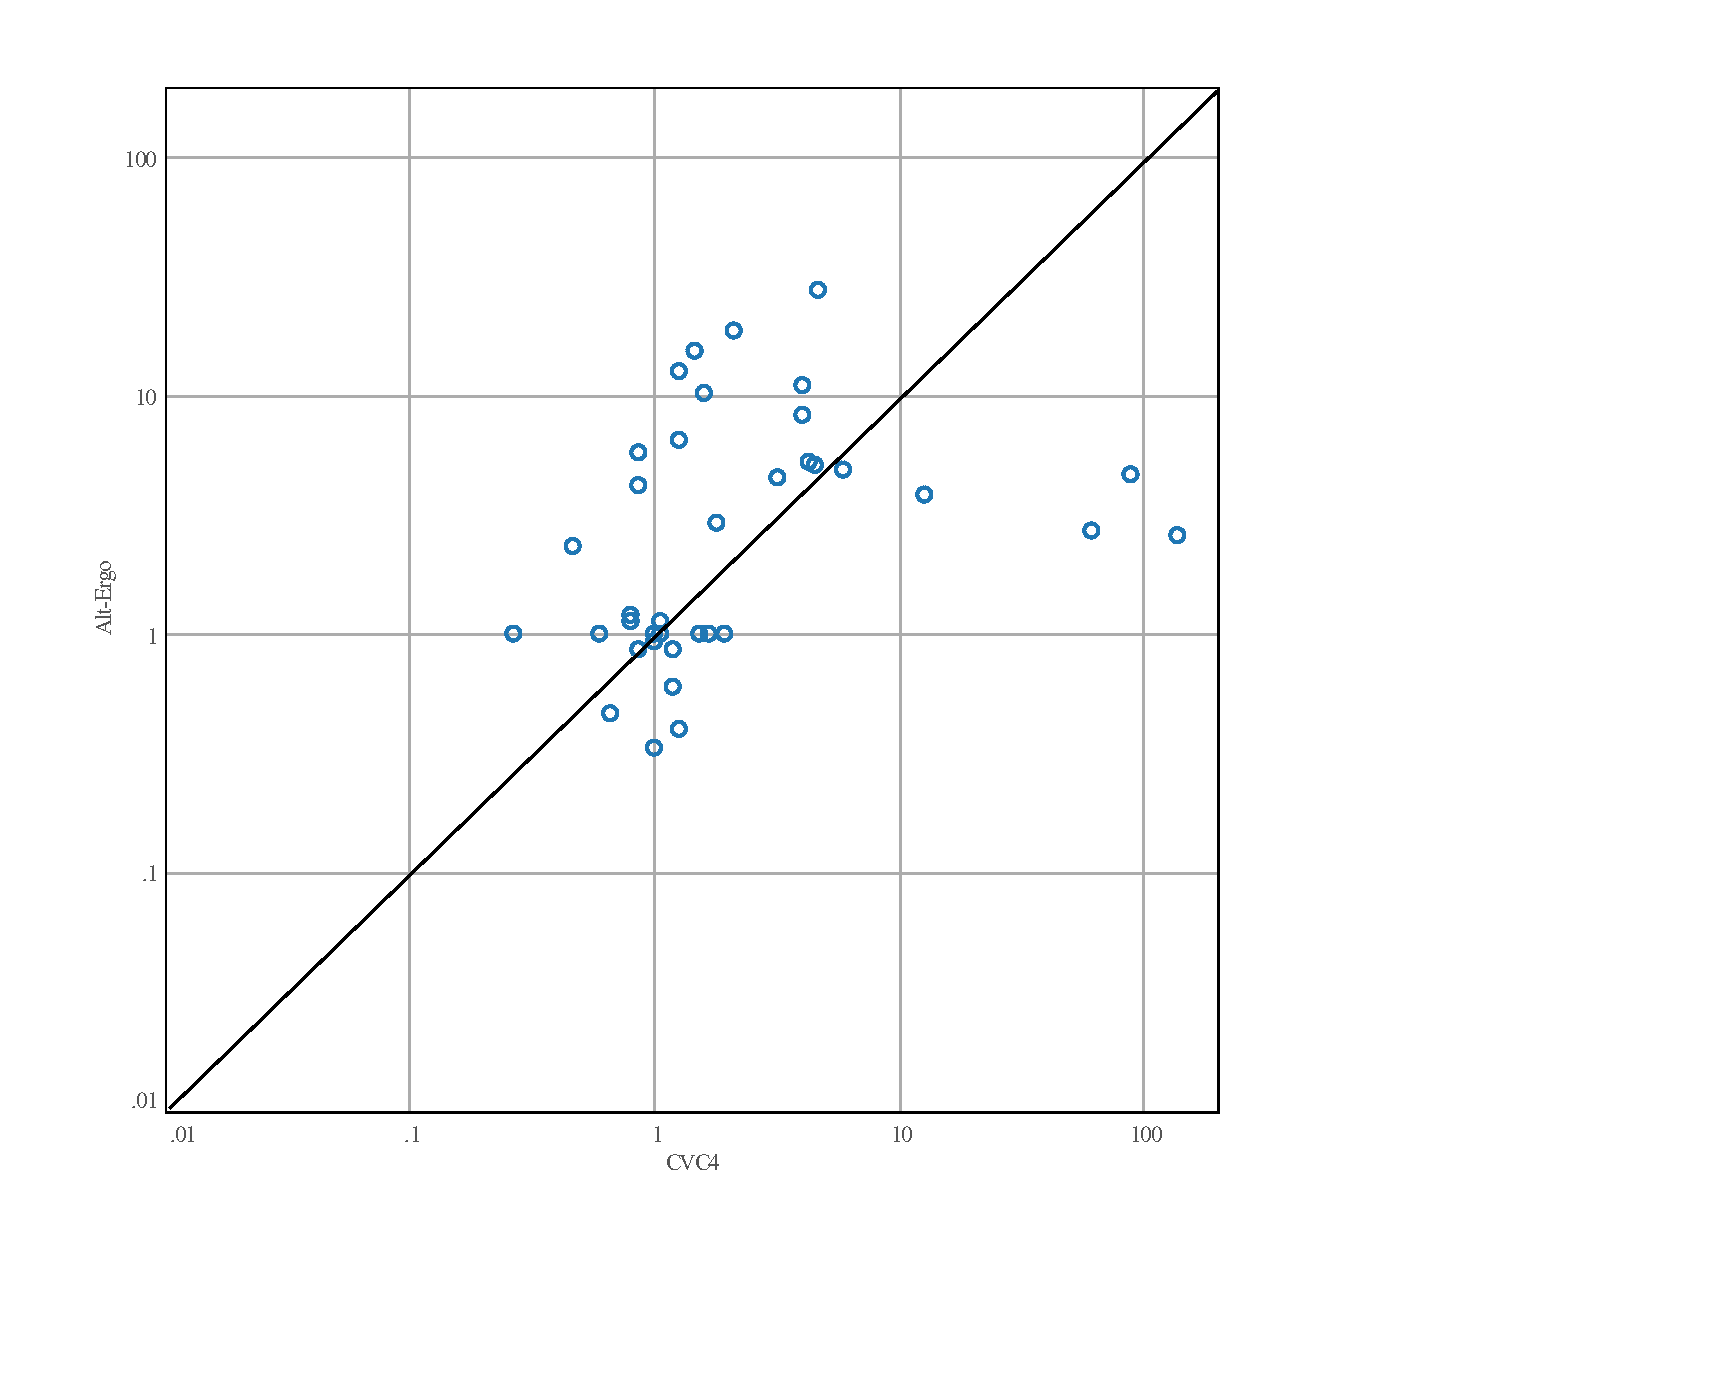
\includegraphics[scale=0.5]{./testanalysis/ScatterInduction.pdf}
\caption{BMC and $k$-Induction Problems (correct answers per second)}
\label{f:ind}
\end{figure}



\section{Conclusion}

CVC4 as a DPLL({\it T}) solver, implemented in C++, is very powerful and effective, especially in QF-UF, QF-LIA, QF-UFIDL, and QF-UFLIA. It works in QF-BV, QF-UFBV and QF-IDL, but not well enough. It has limited support for QF-NIA, and even more limited for UFNIA. It is very efficient in all divisions except QF-BV.

In other words, its theory implementation for free functions and linear integer arithmetic are particularly good. Bit-vectors theory is not as good as previous ones, and quantifiers and non-linear arithmetic are not supported well.

It has good enough support for BMC and $k$-induction problems, which means it has the capability to apply inductive axioms very well.

CVC4 handles large inputs very well, even for input formulas with more than 500 variables and bindings.

Alt-Ergo as a CC(X) solver, implemented using functional language OCaml, performs good in QF-UF. It supports its own Why3 input language, but only supports SMT-LIB 2.0 in a very limited way. According to its performance, it should be good in QF-IDL, QF-UFLIA as well, if it can translate SMT-LIB language better. It runs relatively good enough in UFNIA division, which may due to its AC(X) theory that can quickly solve some non-linear integer arithmetic that only involves associative and commutative properties.

In BMC and $k$-induction problems, Alt-Ergo performs very well, which reflects the fact that it is designed for program verification. It has a very good ability to apply inductive axioms.

Alt-Ergo has problems dealing with large input, which is partly due to the case that it is implemented using a functional language OCaml. Compared to C++, OCaml is not good at memory management, which causes Alt-Ergo to run out of memory a lot.

Comparing the two solvers, CVC4 wins in both capabilities and efficiency. Its solvable problems are a superset of Alt-Ergo's. And Alt-Ergo can't handle {\tt sat} input. But Alt-Ergo performs good enough considering that CVC4 is implemented in C++ while Alt-Ergo is in OCaml.

\section{Integrating CVC4 and Alt-Ergo}

Based on our tests, we found that it is not worth enough to integrate them into one solver. Therefore, we implemented a C frontend that calls both solvers using SMT-LIB scripts, and return the first {\tt sat/unsat} response and kills the other solver. The solver is neither more powerful nor more efficient as expected, which is nearly identical to CVC4 alone.

\section{Future Work}

Currently, we do not have benchmarks in Why3 format, which is the native language for Alt-Ergo. But we plan to contact the authors of Alt-Ergo to get more detailed information of it. Alt-Ergo demonstrats good ability in solving verification related problems in free theory and linear arithmetic. We believe it has good enough potential ability in its native language.

For bit-vectors, CVC4 does not perform very well, and we plan to investigate the reason more carefully in the future.

For those exceptions happened in the tests, we still have some unresolved parts, which needs more time to get a response from the authors of provers. We plan to follow up with those authors to clearify them.

\section{Acknowledgements}

We would like to thank Professor Assaf Kfoury, and Andrei Lapets, who gave us the big picture of this area, and helped answer important questions on $k$-induction. Also thank William Blair and Yilei Chen, who constantly exchanged ideas with us. Without all of your help, we can't get it done smoothly.

\twocolumn
\begin{figure}
\centering
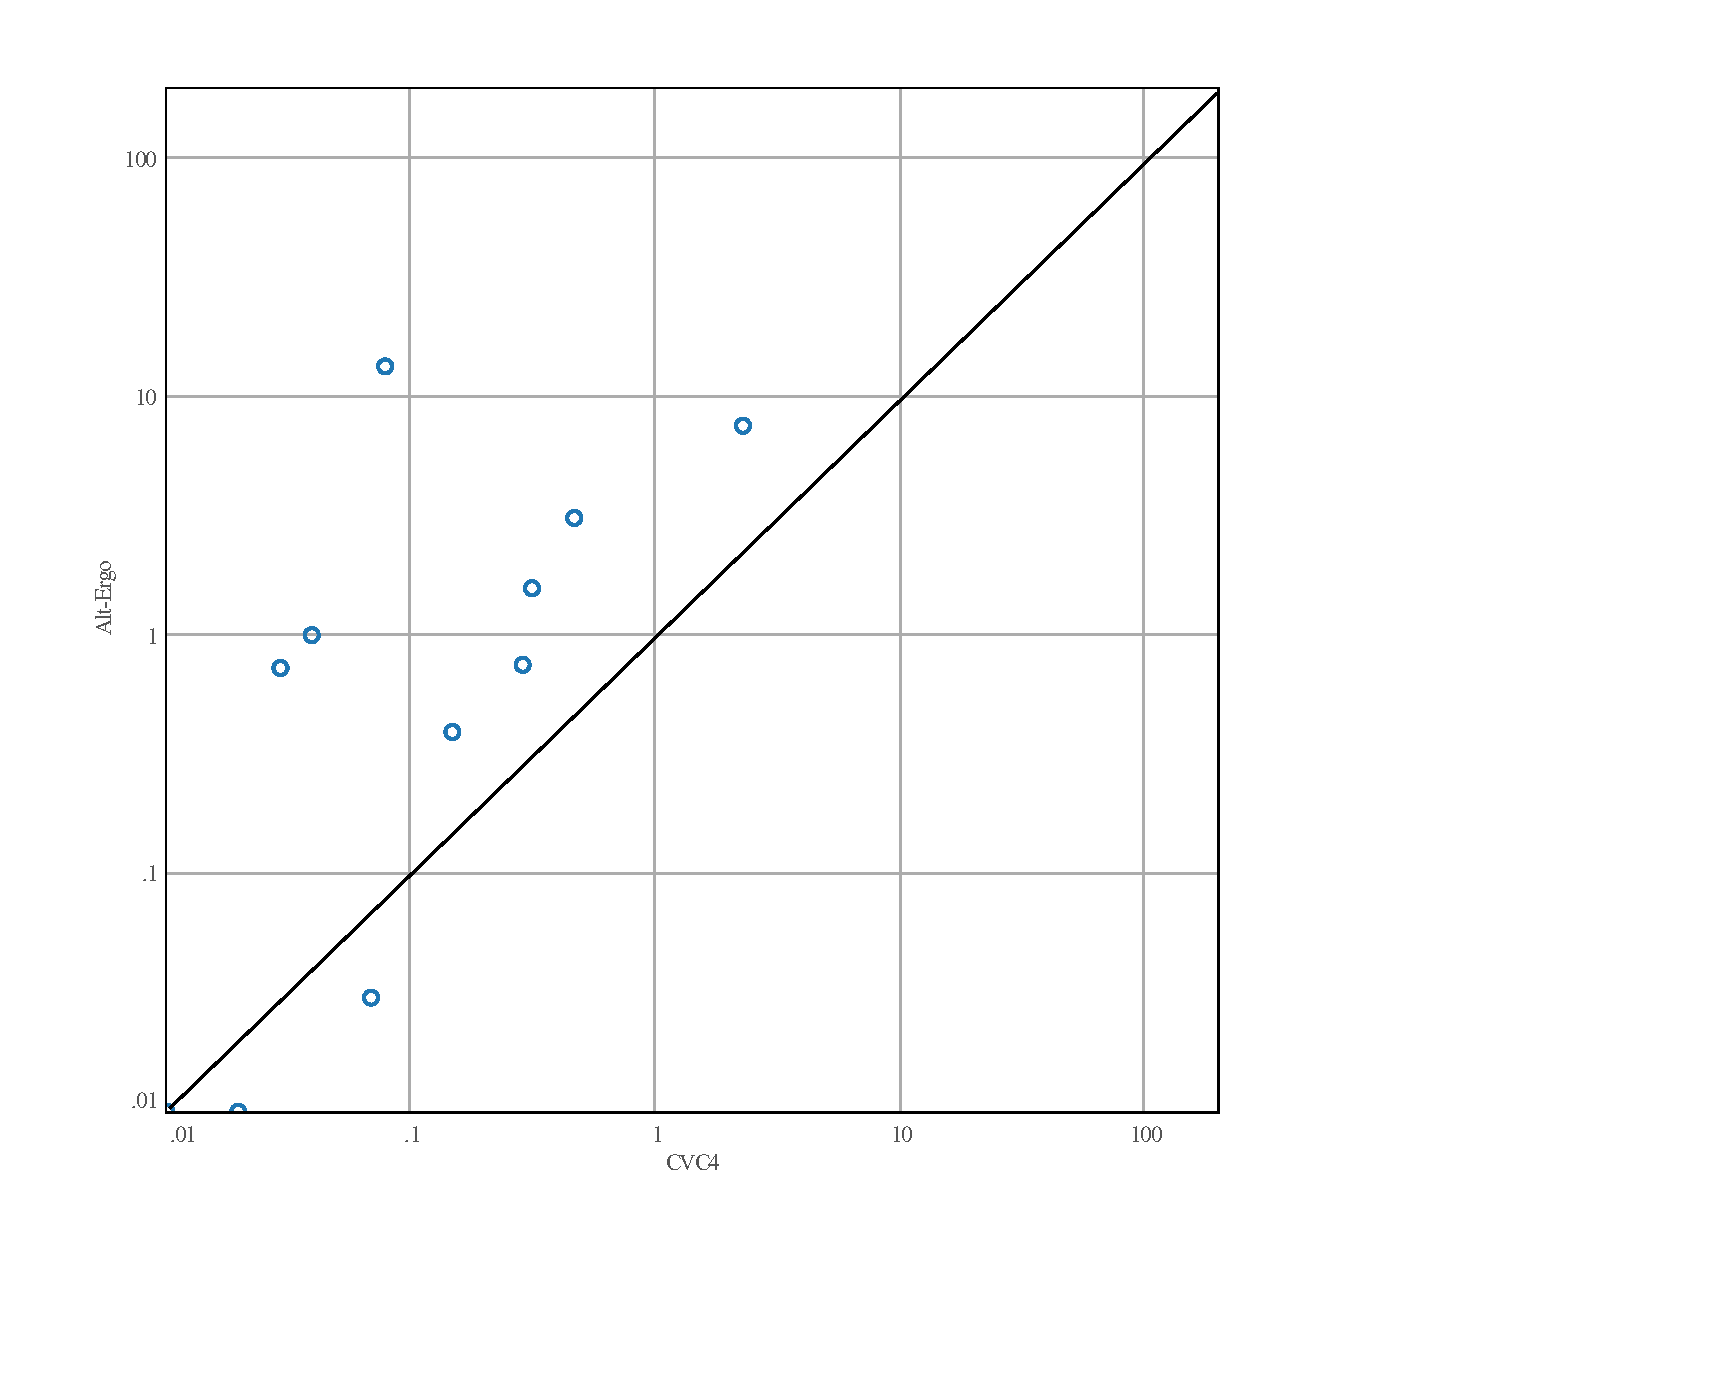
\includegraphics[scale=0.42,trim=0.6cm 0 0 0,clip=true]{./testanalysis/ScatterQFIDL.pdf}
\caption{QF-IDL (avg. time, log scale)}
\label{f:qfidl}
\end{figure}

\begin{figure}
\centering
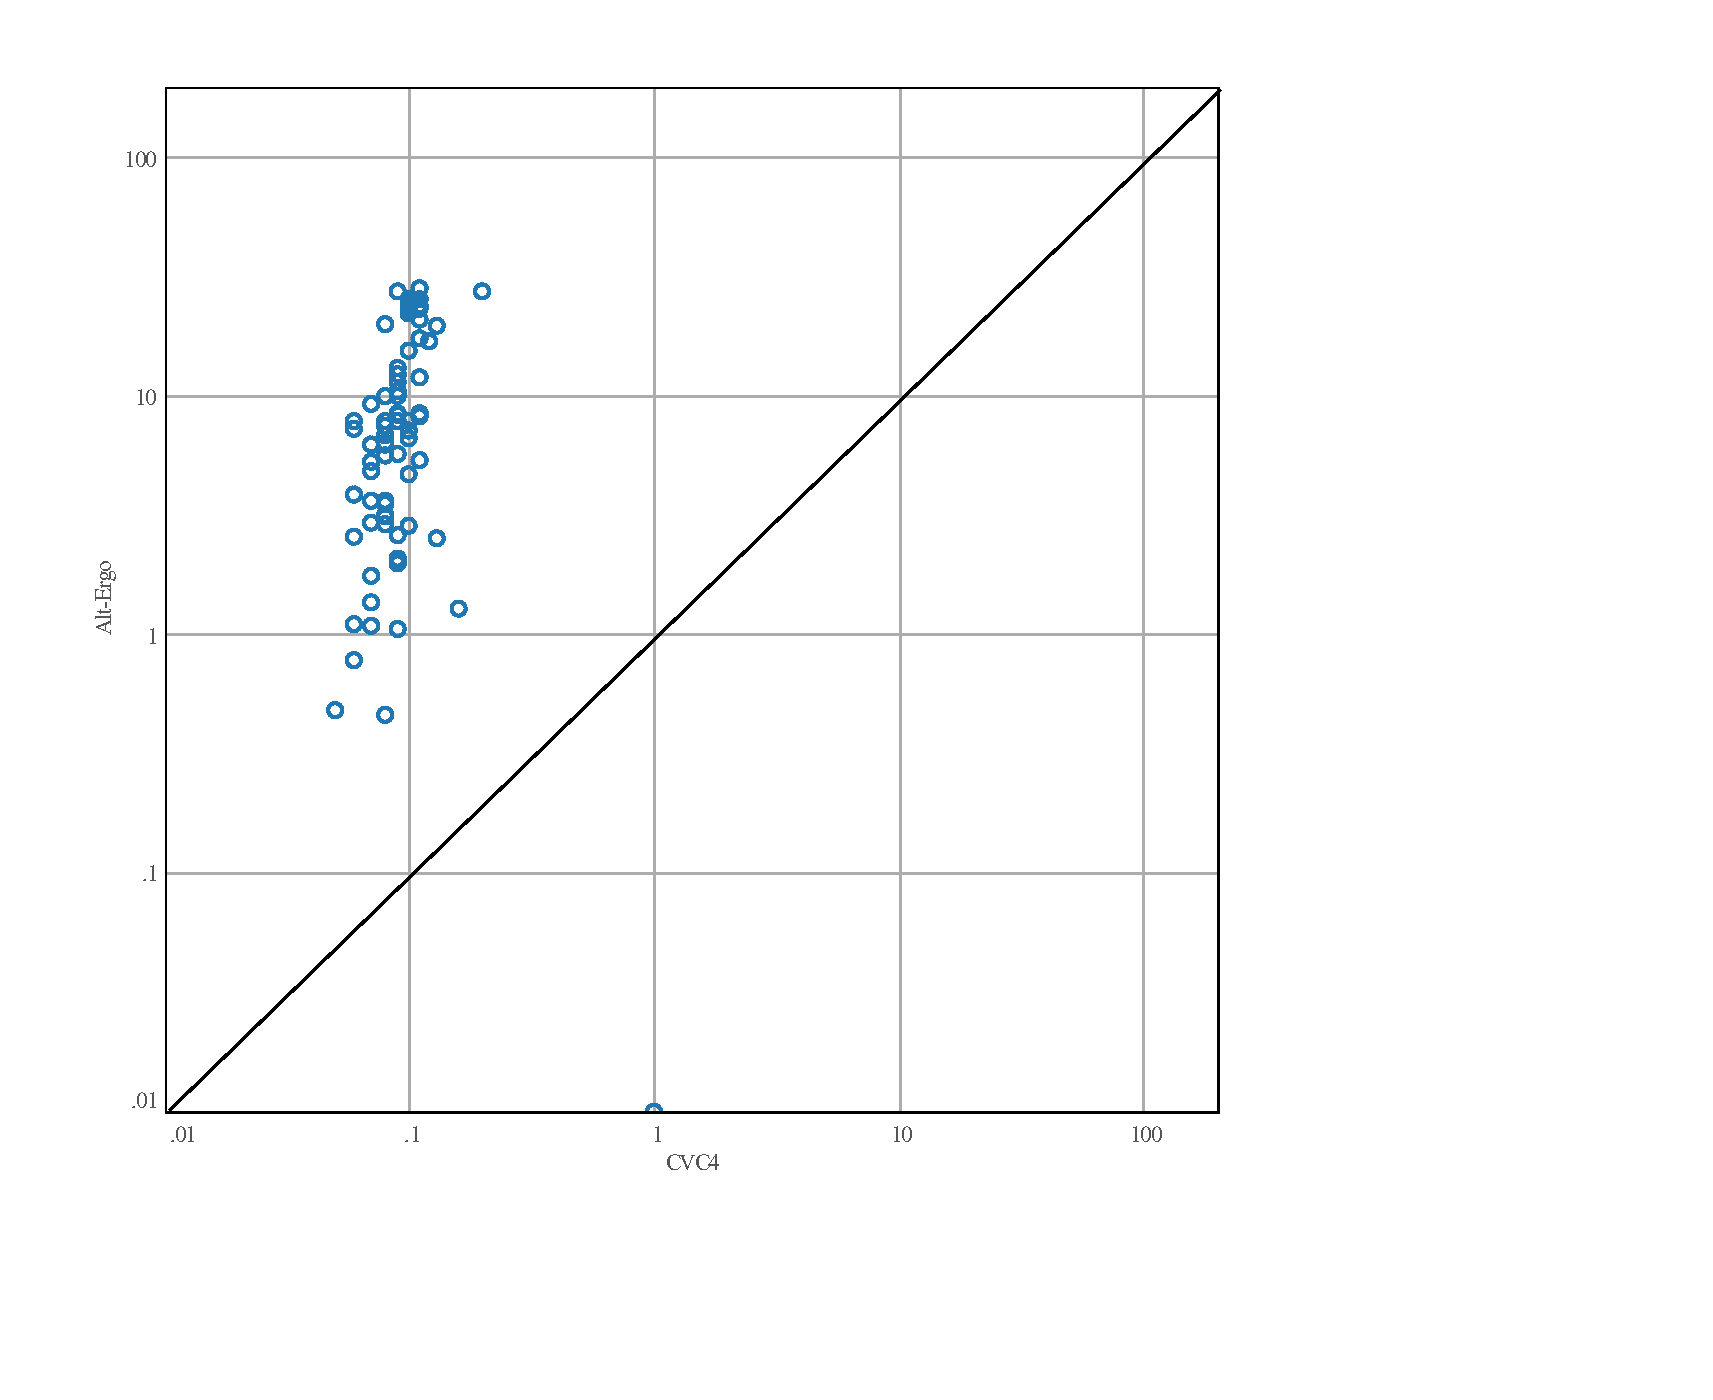
\includegraphics[scale=0.42,trim=0.6cm 0 0 0,clip=true]{./testanalysis/ScatterQFUF.pdf}
\caption{QF-UF (avg. time, log scale)}
\label{f:qfuf}
\end{figure}

\begin{figure}
\centering
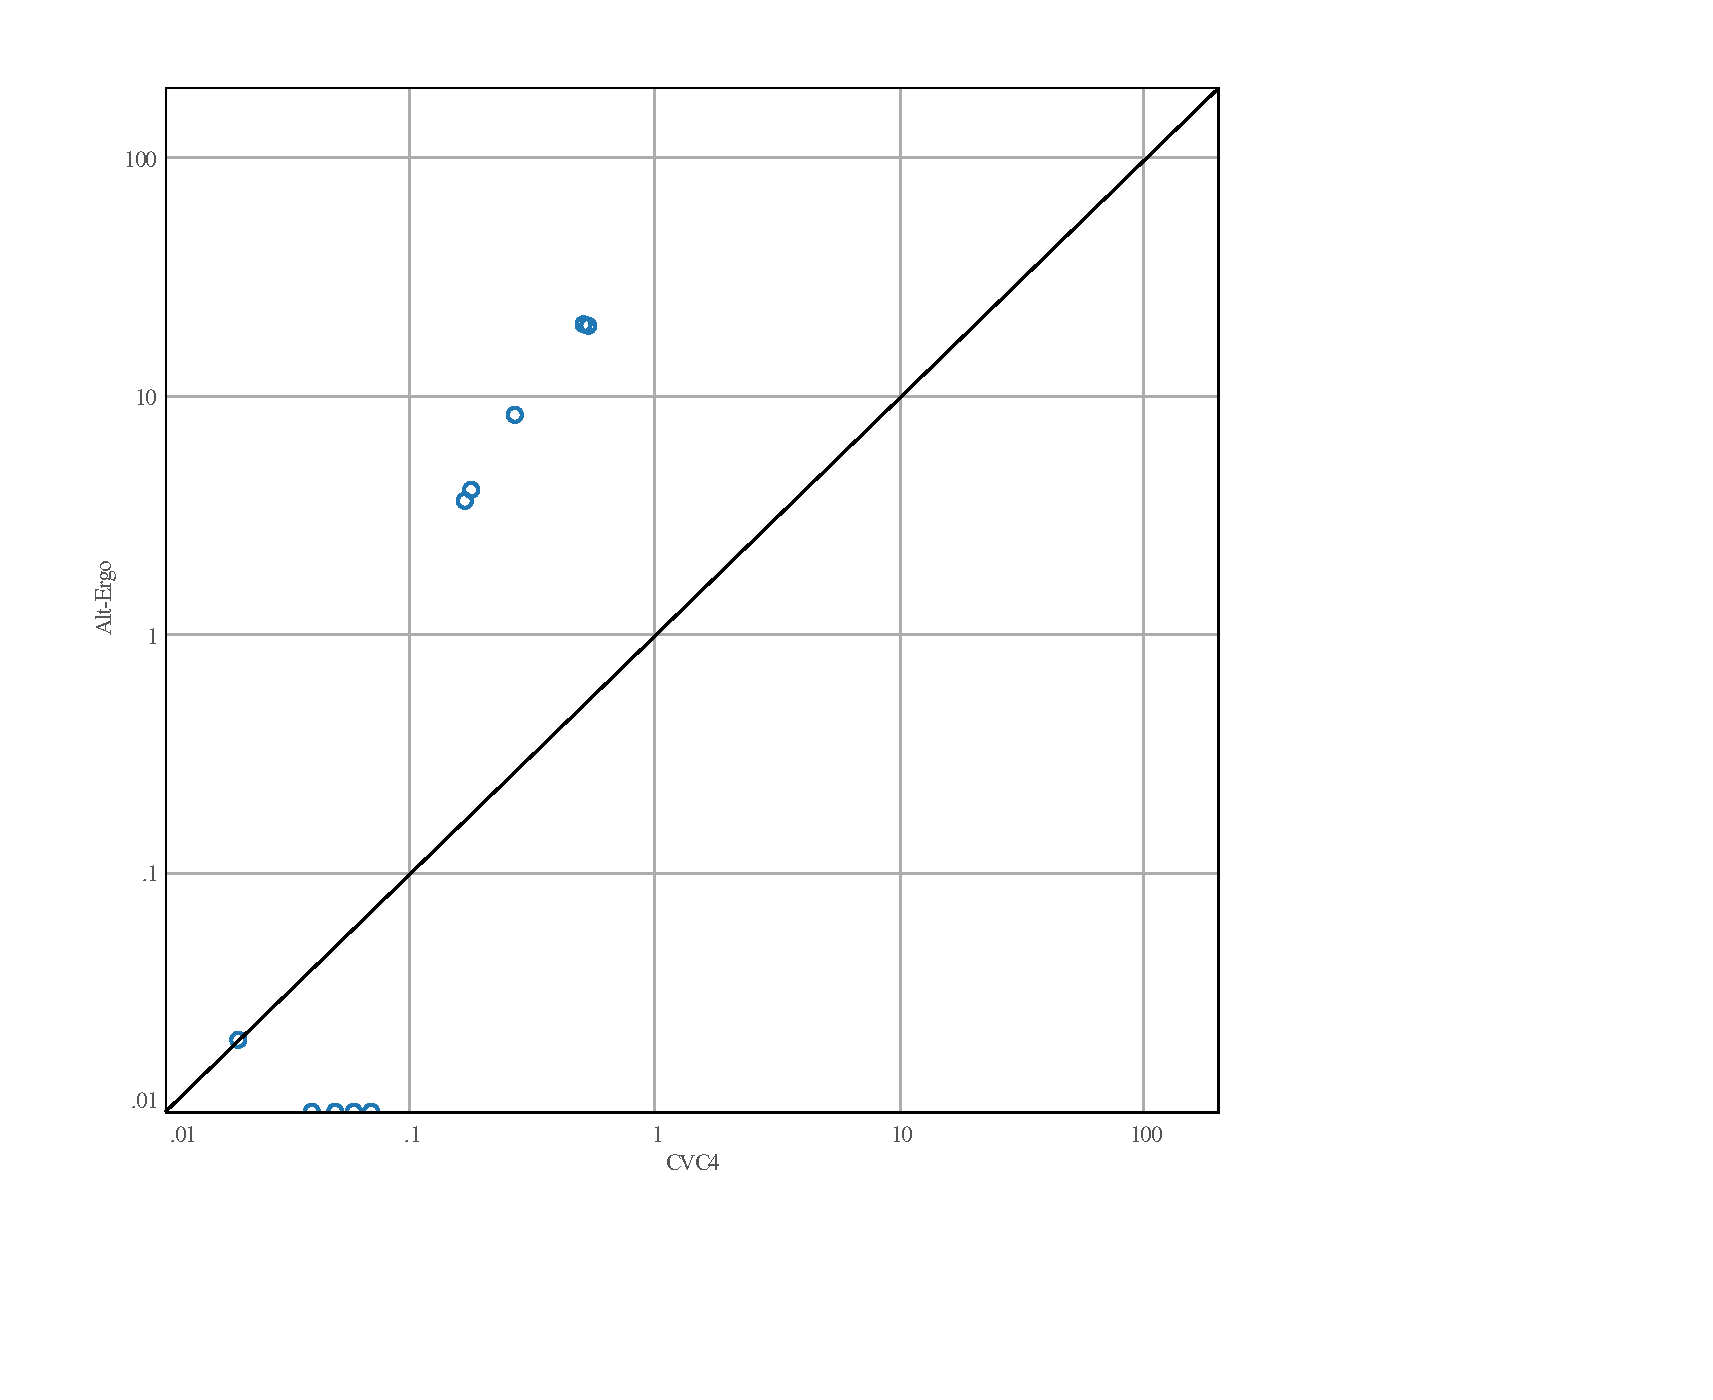
\includegraphics[scale=0.42,trim=0.5cm 0.5cm 0 0, clip=true]{./testanalysis/ScatterQFUFLIA.pdf}
\caption{QF-UFLIA (avg. time, log scale)}
\label{f:qfuflia}
\end{figure}

\begin{figure}
\centering
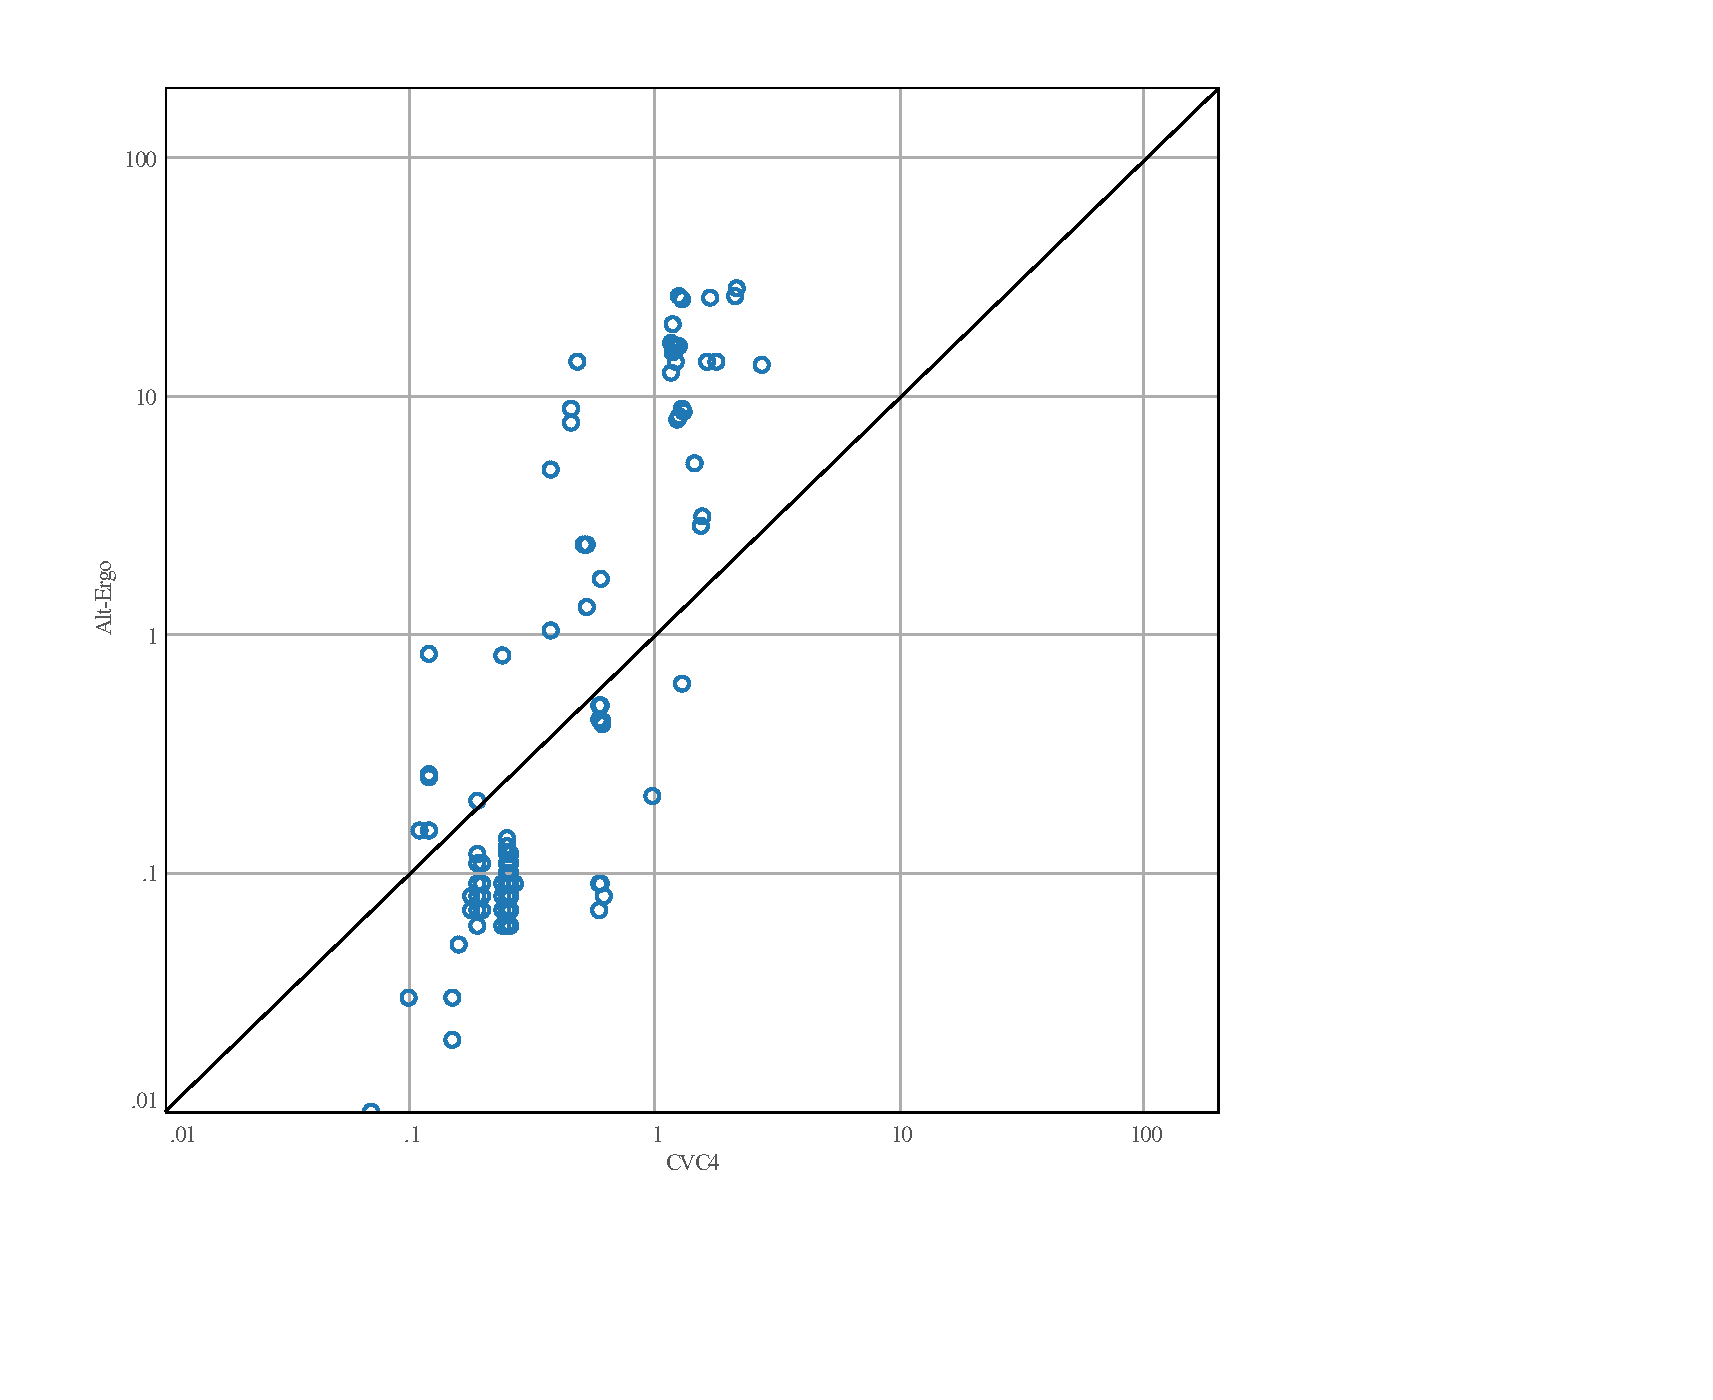
\includegraphics[scale=0.42,trim=0.5cm 0.2cm 0 0, clip=true]{./testanalysis/ScatterUFNIA.pdf}
\caption{UFNIA (avg. time, log scale)}
\label{f:ufnia}
\end{figure}

\onecolumn


\twocolumn
\begin{sidewaysfigure}
\centering
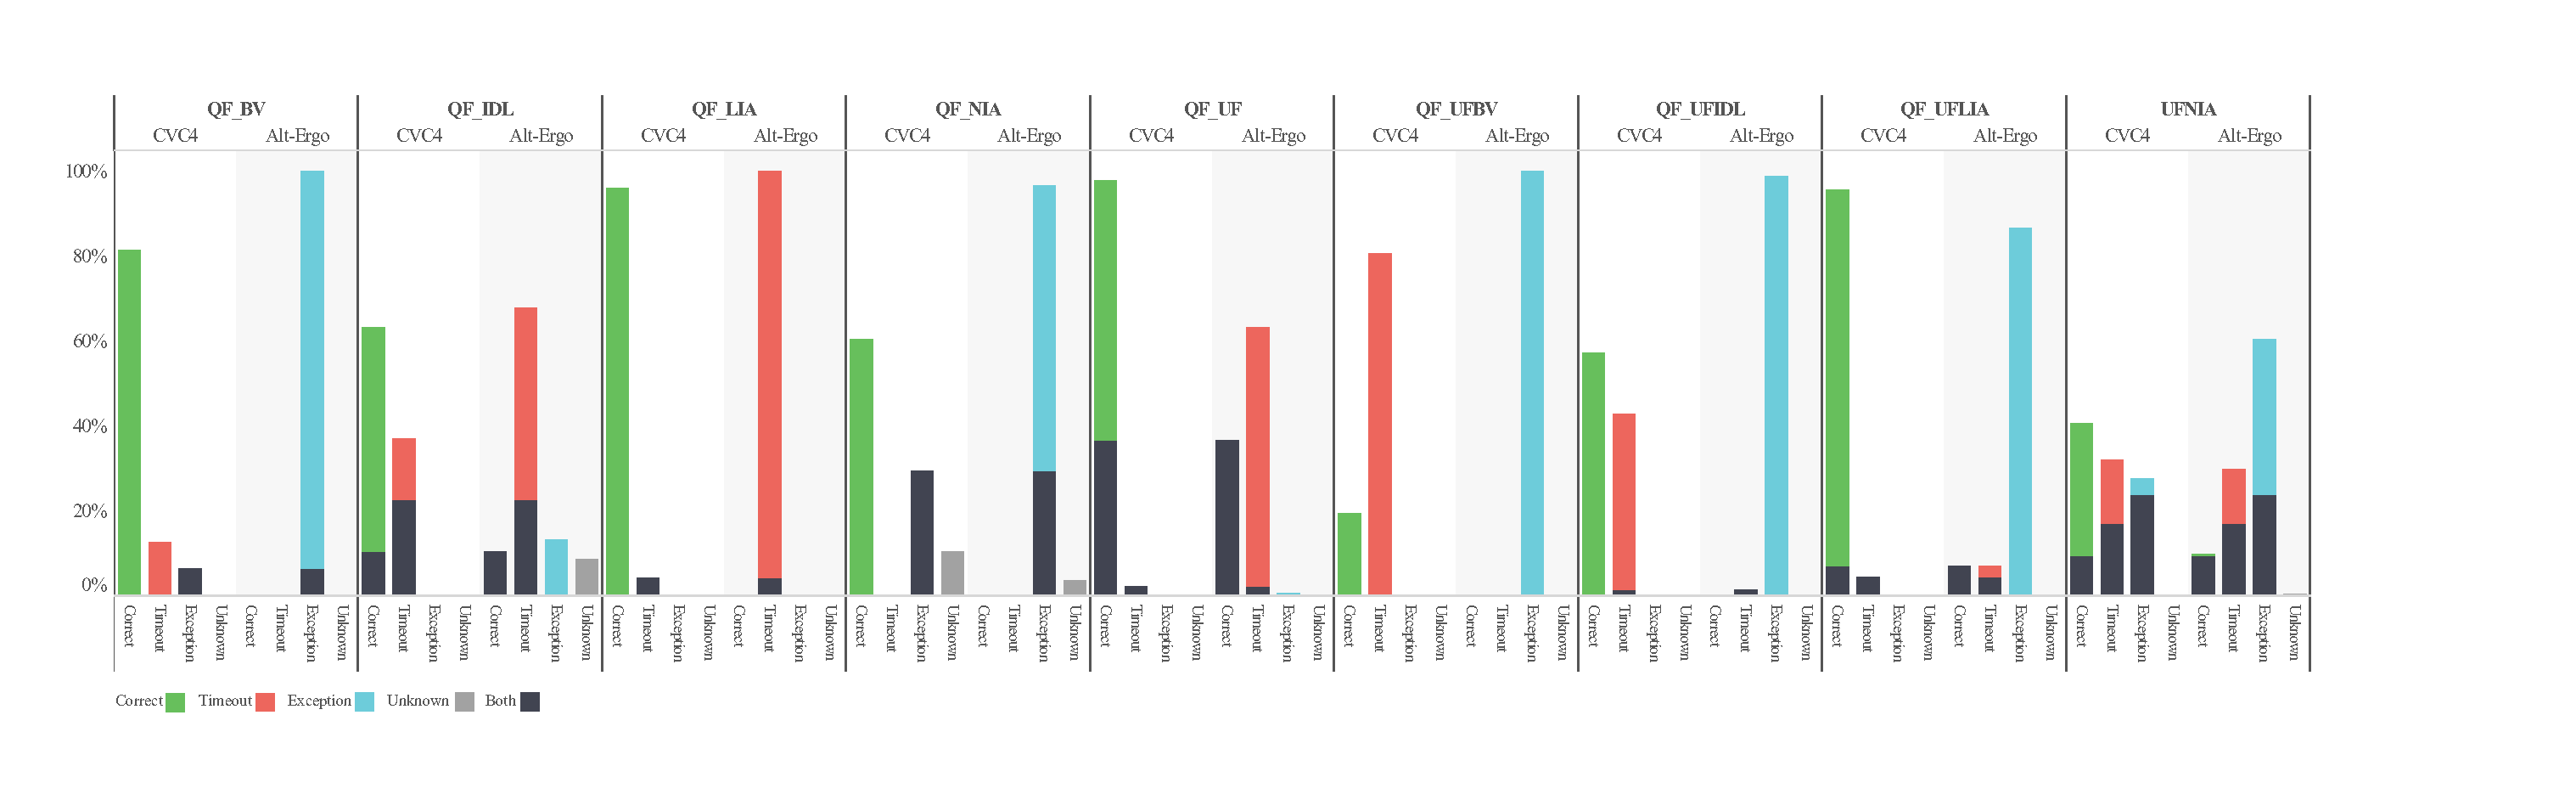
\includegraphics[scale=0.45]{./testanalysis/unsatcap.pdf}
\caption{Capabilities of CVC4 and Alt-Ergo on {\tt unsat} Tests}
\label{f:unsatcap}
\end{sidewaysfigure}


\begin{sidewaysfigure}
\centering
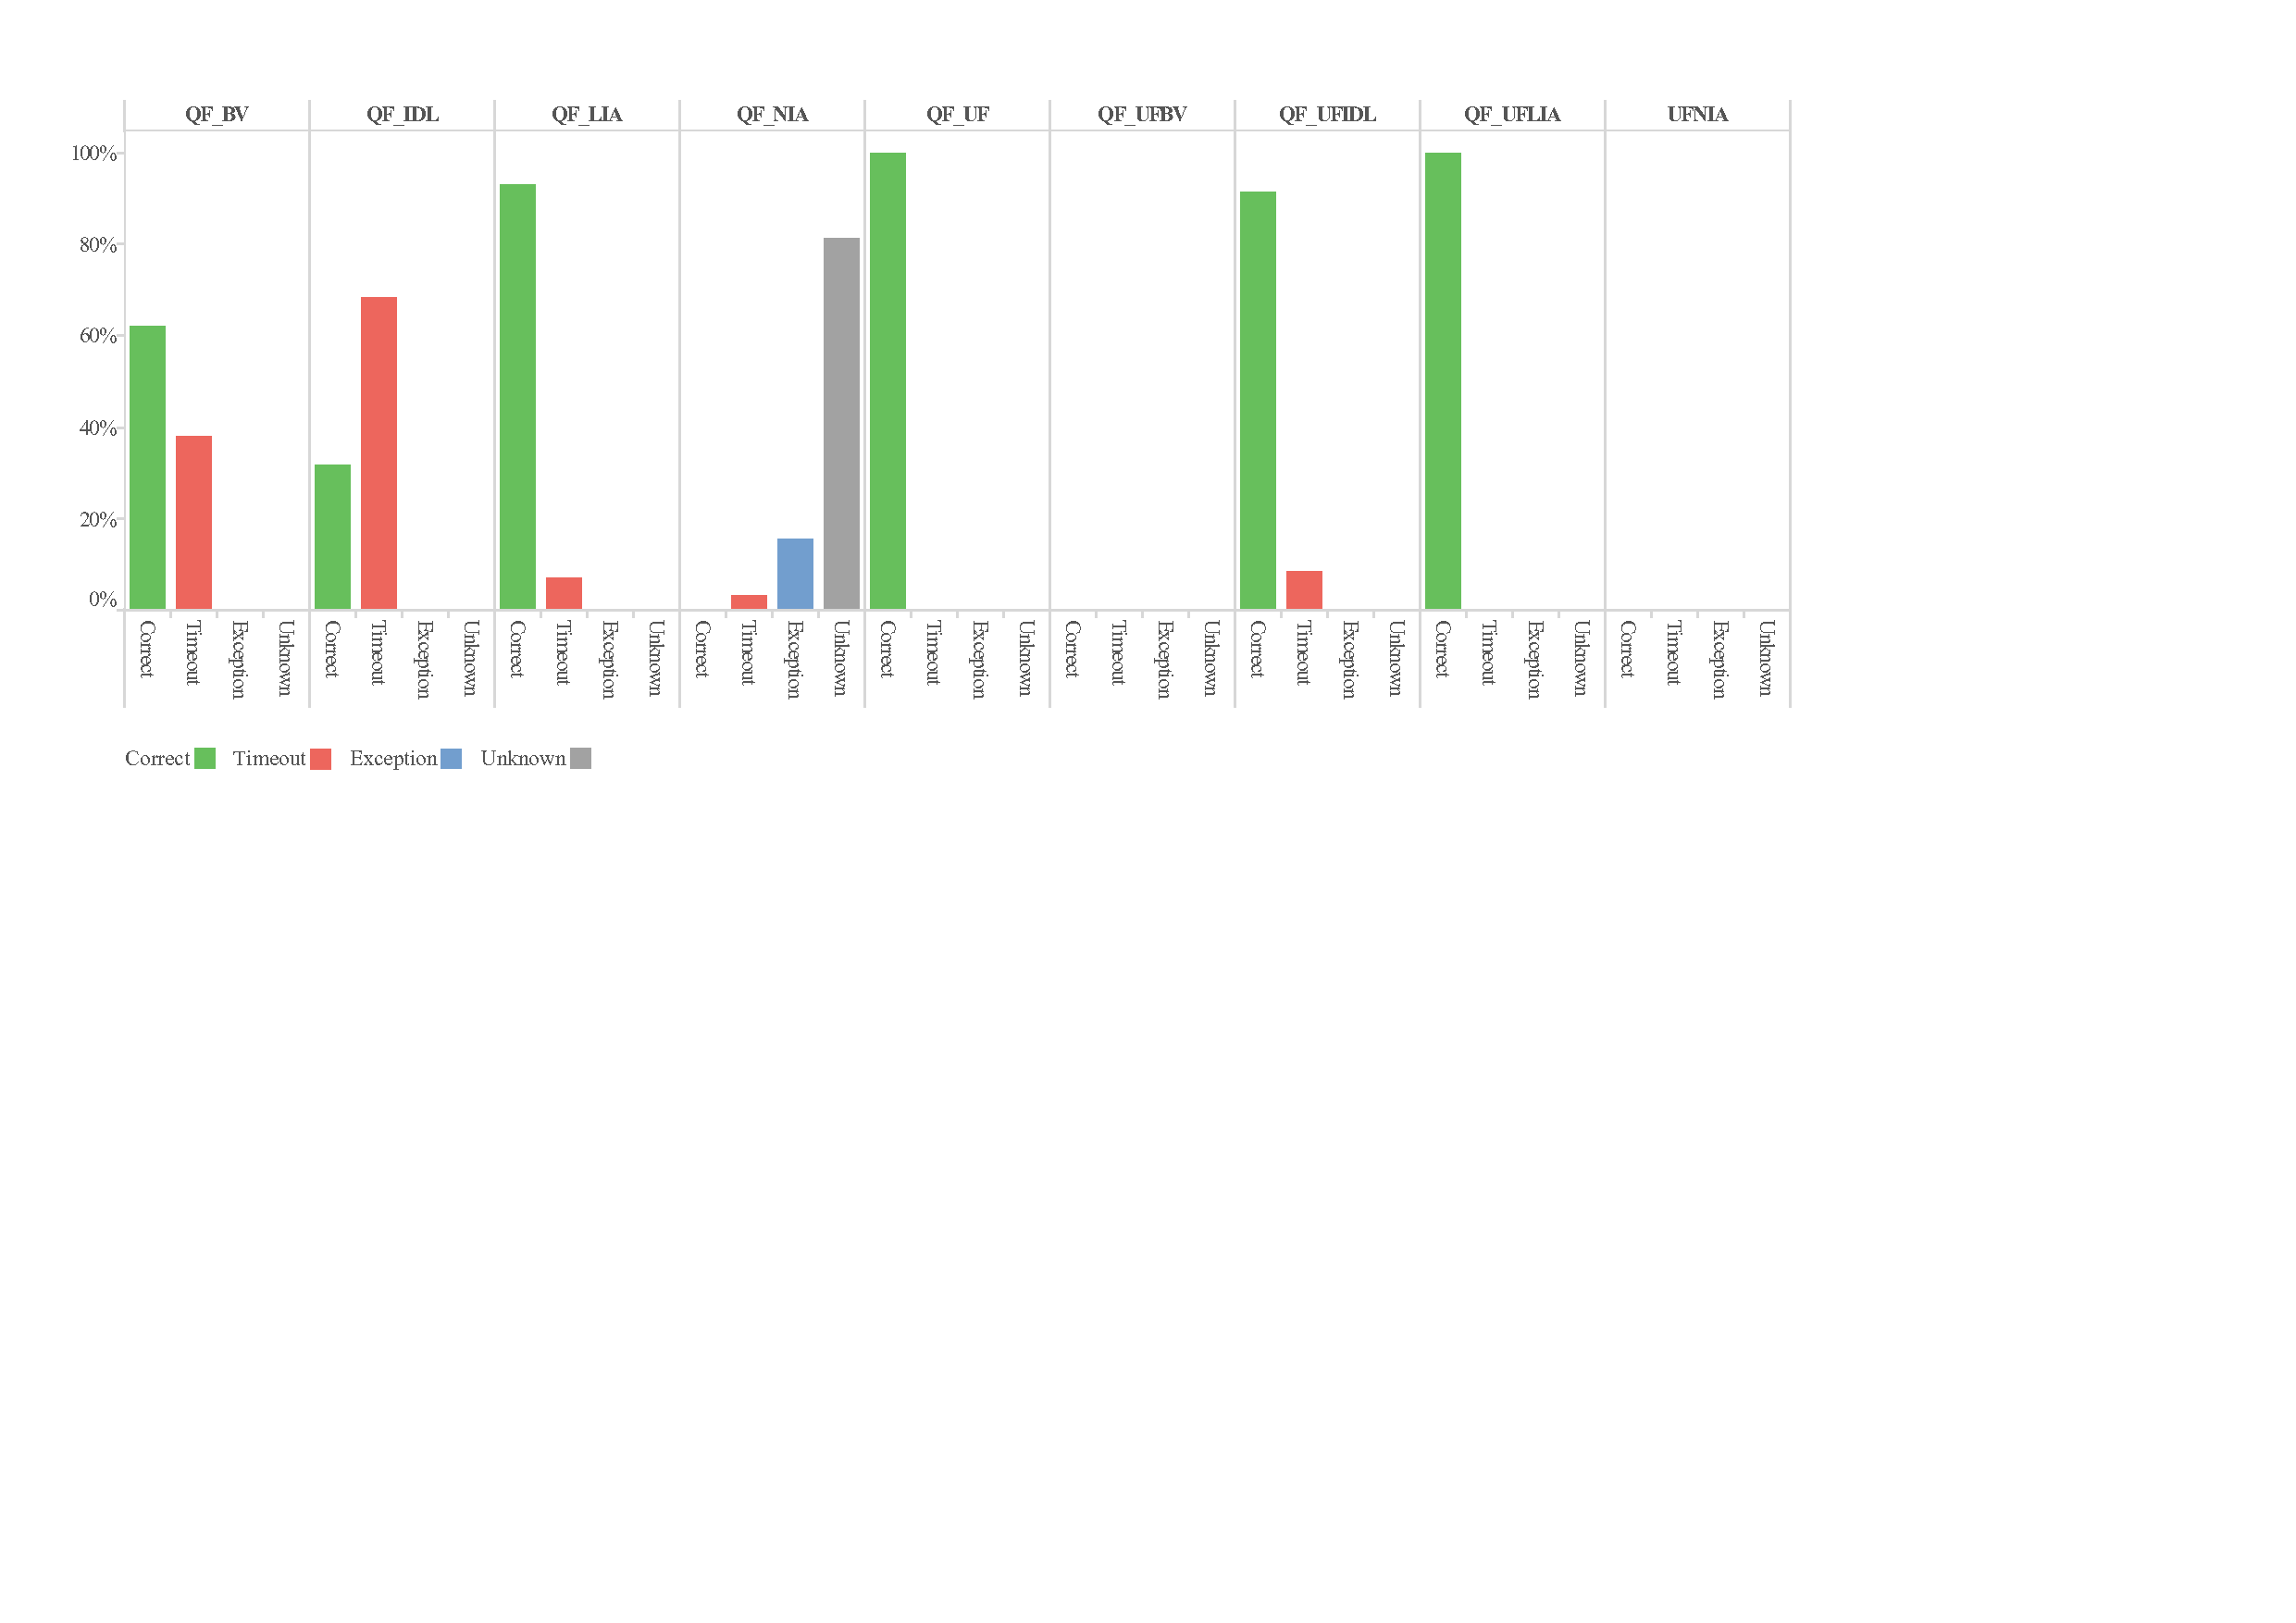
\includegraphics[scale=0.45]{./testanalysis/satcap.pdf}
\caption{Capabilities of CVC4 on {\tt sat} Tests}
\label{f:satcap}
\end{sidewaysfigure}

\onecolumn






\bibliographystyle{alpha}
\bibliography{smtlib}


\end{document}



